% EPL master thesis covers template
\documentclass{eplmastersthesis}
\usepackage{float}
\usepackage{xcolor}
\usepackage{listings}
\usepackage{hyperref}
\usepackage[final]{graphicx}
\usepackage{subcaption}
\usepackage{csquotes}

\setcounter{secnumdepth}{4}
\setcounter{tocdepth}{4}

\lstdefinestyle{MyLua}{
  language         = [5.3]Lua,
  basicstyle       = \small\ttfamily,
  keywordstyle=\color{magenta},
  stringstyle=\color{blue},
  commentstyle=\color{black!50},
  frame=single,
  tabsize=2,
  showspaces=false,
  showstringspaces=false,
  literate={\ \ }{{\ }}1
}

\lstdefinestyle{MySmallLua}{
  language         = [5.3]Lua,
  basicstyle       = \tiny\ttfamily,
  keywordstyle=\color{magenta},
  stringstyle=\color{blue},
  commentstyle=\color{black!50},
  frame=single,
  tabsize=2,
  showspaces=false,
  showstringspaces=false,
  literate={\ \ }{{\ }}1
}

\lstdefinestyle{MyBash}{
  language = bash,
  basicstyle=\scriptsize\ttfamily,
  showstringspaces=false,
  commentstyle=\color{red},
  keywordstyle=\color{blue},
  showspaces=false,
  showstringspaces=false
}

\lstdefinelanguage{Log}{
  keywords={}
}

\lstdefinestyle{MyLog}{
  language = Log,
  basicstyle=\scriptsize\ttfamily,
  numbers=left,
  frame=single
}


% Please fill in the following boxes
% Title of the thesis
\title{Integrated platform for distributed systems training}

% Subtitle - remove this line if not applicable
\subtitle{The Splay Project}

% Name of the student author(s)
\author{Rémy \textsc{Voet}}
\secondauthor{Samuel \textsc{Monroe}}		% remove if not applicable
%\thirdauthor{Firstname \textsc{Lastname}}			% remove if not applicable

% Official title of the master degree (copy/paste from list below)
% Master [120] in Biomedical Engineering
% Master [120] in Chemical and Materials Engineering
% Master [120] in Civil Engineering
% Master [120] in Computer Science
% Master [120] in Computer Science and Engineering
% Master [120] in Cybersecurity
% Master [120] in Data Sciences Engineering
% Master [120] in Data Science: Information technology
% Master [120] in Electrical Engineering
% Master [120] in Electro-mechanical Engineering
% Master [120] in Mathematical Engineering
% Master [120] in Mechanical Engineering
% Master [120] in Physical Engineering
% Master [60] in Computer Science
% Specialised master in nanotechnologies
% Specialised master in nuclear engineering
\degreetitle{Master [120] in Computer Science}

% Name of the supervisor(s)
\supervisor{Étienne \textsc{Rivière}}
\secondsupervisor{Raziel \textsc{Carvajal Gomez}}		% remove if not applicable
%\thirdsupervisor{Firstname \textsc{Lastname}}		% remove if not applicable

% Name of the reader(s)
\readerone{Guillaume \textsc{Derval}}
\readertwo{Raziel \textsc{Carvajal Gomez}}			% remove if not applicable
\readerthree{Peter \textsc{Van Roy}}			% remove if not applicable
%\readerfour{Firstname \textsc{Lastname}}			% remove if not applicable
%\readerfive{Firstname \textsc{Lastname}}			% remove if not applicable

% Academic year (update if necessary)
\years{2018--2019}

% Document
\begin{document}
  % Front cover page
  \maketitle

  \chapter*{Abstract}

    

  \chapter*{Acknowledgements}

    We would like to thank Etienne Riviere, our thesis supervisor who offered
    us the opportunity of working on this project and took some precious time
    to hold a meeting with us each week during two whole semesters.\\

    We also thank Raziel Carvajal Gomez for helping us during our
    part-time job period on the Splay application.\\

    Finally, we thank Peter Van Roy and Guillaume Derval for taking the time
    of being readers of our thesis.

  \tableofcontents

  \chapter{Introduction}

    Distributed algorithms are at the core of applications in domains as
    various as cloud computing, networking or artificial
    intelligence~\cite{DistributedArtificialIntelligence}.\\
    An algorithm is distributed when it is designed to run on several
    processors or machines linked by a network, achieving a common task
    or dividing a workload processing.\\

    As we start pursuing the development of distributed applications,
    we start encountering specific problems:
    \begin{itemize}
      \item How should the application handle network issues such as
      a network partition due to a failing link, or how should the application
      behave in extreme conditions with low quality connections between
      the nodes?
      \item How should the application handle nodes failures among the
      collection of nodes achieving the common task? How it should handle
      nodes crashing then restarting?
    \end{itemize}

    \section{Learning Distributed Algorithms}

      The process of learning distributed algorithms is usually by the
      difficulty of being able to test and apply what one learns.\\
      Usually, students are learning the theoretical components of the
      algorithms (consensus, leader election, resource allocation, ...)
      and if ever they want to start practically learning with a real
      implementation to deepen their knowledge, some practical problems
      start to appear:

      \begin{itemize}
        \item The first issue comes from the nature of the algorithms: they are
        distributed. This means a student will need to setup a testing
        environment by deploying or simulating a collection of machines on
        which he would run his algorithm implementation.
        \item This collection of machines needs to be set up, each machine has
        to communicate with each other in order to achieve their common task.
        \item The student will also need to get feedback on how his
        algorithm performed.
        \item The student will implement the algorithm from pseudo-code
        \footnote{Pseudo-code is an informal and simplified programming language}
        and will be confronted to one of the following problems when setting
        communication and feedback on the machines:
          \begin{itemize}
            \item He will bloat his implementation with all the needed
            code for communication and feedback.
            \item He will spend a lot of time implementing a complex
            system to achieve communication and feedback behind the scenes if
            trying to avoid the previous problem.
          \end{itemize}
        Either way, it will be a cause of errors unrelated to its
        implementation and will drag him out of his main goal of learning
        distributed algorithms.
        \item Distributed algorithms are designed to have resilience
        properties in cases of node crashes or other events. How the student
        could experiment what should happen when a node dies? This will result
        in even more code bloating or in an even more complex home-made system.
      \end{itemize}

      Another issue with distributed algorithms is that the pseudo-code
      (from papers for example) is usually far from what a true solution to the
      related problem would be. There is in general a lot of time management
      and asynchronous calls and responses from the nodes among the system,
      increasing the gap between the theoretical specifications and practical
      cases.

    \section{Learning Solutions}

      There is a need for solutions to help students in the distributed
      algorithm learning process.\\

      Some testbeds facilitate the testing of distributed algorithms, such as
      \texttt{emulab}~\cite{Emulab}, \texttt{ModelNet}~\cite{ModelNet} or
      \texttt{PlanetLab}~\cite{PlanetLab}. But these solutions have some serious
      drawbacks:

      \begin{itemize}
        \item They are quite complicated to use and hard to learn
        \item They are difficult to install or deploy
        \item They mostly only address the problem of setting up a collection
        of nodes
      \end{itemize}

      Concerning the code itself, supplying a high level library helping the
      creation of distributed algorithms is a possible solution. Some
      exists for that precise purpose in different languages, such as:

      \begin{itemize}
        \item \texttt{Mace}~\cite{Mace} in \texttt{C++}
        \item \texttt{Pymote}~\cite{Pymote} in \texttt{Python}
      \end{itemize}

      These solutions were not integrated together or not suiting the real needs
      for making the development of distributed algorithms easier and better,
      thus offering a place for a better solution that would be:

      \begin{itemize}
        \item Focused around the development of the algorithm;
        \item Allowing simulation of real-life conditions;
        \item Easy to use and install for any user;
        \item Light enough for low costhardware.
      \end{itemize}

      This is where the \texttt{Splay} project takes its origins.

    \section{Splay}

      The \texttt{Splay} project was initiated to solve the difficulty to test
      and develop distributed algorithm in a large scale. \texttt{Splay} is
      not a recent project (started around 2006), and lot of features have been
      added since it's creation. The first version of \texttt{Splay} was
      designed to "cover all aspects of the development and evaluation
      chain" of distributed application~\cite{SPLAY}.\\
      After some years a module has been developed to emulate network
      topologies, \texttt{SplayNet}~\cite{SplayNet}. This middleware implements
      an easy way to set the topology network between the endpoints (machines)
      and emulate the behaviour in latency, throughput and congestion according
      to that topology.

    \section{Our Work on Splay}

      Our thesis details our work on the \texttt{Splay} project. \texttt{Splay}
      was initially designed to be used by researchers in distributed systems,
      our goal was to enhance the initial project to turn it into a framework
      better suited for teaching and learning.\\
      This work follows the idea of providing students with tools
      allowing them to practically assess what they learn during the
      theoretical lessons, as the \texttt{INGInous}~\cite{inginious} platform allows.\\
      As their \texttt{Github} repository explains :
      \begin{displayquote}
        "\texttt{INGInious} is an intelligent grader that allows secured and
        automated testing of code made by students."
      \end{displayquote}
      We think that our work is complementary to what \texttt{INGInous} achieves,
      bringing new ideas and solutions on the distributed systems learning
      side.\\

      We relaunched the development of \texttt{Splay}, starting from a stable
      version and progressively updating it and adding new
      features in order to make it a good tool for the learning and
      experimentation of distributed algorithms.\\
      This tool would be focused around the algorithm itself and allowing to
      perform testing under different conditions about the network or
      the nodes themselves.\\

      We made the following contributions:

      \begin{itemize}
        \item An extensive work of updates and bug fixes on the base project.
        \item Changes in the software and services architecture of \texttt{Splay},
        including rewriting some services, to propose an easier to maintain and
        more testable project.
        \item Deep changes on the software engineering side, forking the
        previous project, reorganizing it and setting up quality-enforcement
        best practices like automatic builds and continuous integration.
        \item Ensuring code quality by writing a lot of test suites for the
        different services composing \texttt{Splay}, testing services individually,
        globally and using different techniques of testing (unit testing,
        integration testing, ...).
        \item Enhancing the project with new features designed to provide a
        student with all the necessary environment for an easier and convenient
        way of learning distributed algorithms.
      \end{itemize}

      This document will detail how we turned \texttt{Splay} into an integrated
      platform designed to help students learning and practicing distributed
      systems.\\
      In the next chapter, we will explicit how we designed the changes made on
      \texttt{Splay} to address the problem of making it a learning and teaching
      platform.\\
      Chapter~\ref{chap:dev} will explain in detail all our development,
      implementation and architectural changes on \texttt{Splay}.\\
      Chapter~\ref{chap:qual} will present all our work to ensure code quality
      in the project.\\
      We will then explain the development of the new features
      of \texttt{Splay} in chapter~\ref{chap:newfeat}, present a real scenario
      of usage in chapter~\ref{chap:usercase} and then conclude this document.

  \chapter{Splay for Learning and Teaching}
  \label{chap:splayteaching}

    In this chapter, we will explicit the solution needed to help the
    students learn distributed algorithms, then detail what the previous
    version of \texttt{Splay} was offering.\\
    Based of scenarios describing practical use cases of our solution, we will
    then draw a roadmap of modifications and enhancements we decided to
    contribute to the project.

    \section{A Solution Definition}

      We wanted an application that allows students and professors to develop
      and test distributed algorithms. These are the qualities needed for this
      application:

      \begin{itemize}
        \item The application should be easy to use for beginners and people
        who just started to learn Distributed Systems, but also for professors.
        \item The application should allow the user to define parameters about
        the network and nodes he is running his algorithm on such as latencies
        or packet losses.
        \item The application should provide an practical way for the user
        to write his algorithm.
        \item The application should allow the user to get detailed information
        about how his algorithm performed within the system.
        \item The application should offer services focused on the development
        of algorithm. No time should be spent on the configuration of the
        machines needed to create a distributed system ready to run algorithms.
      \end{itemize}

    \section{What Splay Offered}

      In this section, we will go through specific topics concerning the \texttt{Splay}
      application in the state \textbf{before} we added our contributions.\\
      We will first detail how a user interacted with the application,
      defining in the mean time specific terms related to
      the application and that we will use in the rest of this document with
      the same meaning.\\
      Then, we will detail the software architecture, proposing a global
      picture of the application and then going through each component. This
      part will also detail what happens internally during a user interaction
      with the application.

      \subsection{Application Usage}

        The user is able to interact with the application through two
        services, a command line interface and a full-stack web application.\\
        In order to test a distributed algorithm the user has to send, through
        one of these services, what we call a \textbf{\texttt{job}}. A
        \texttt{job} encapsulates everything needed by the application
        to run the distributed algorithm and is composed of the following
        elements:

        \begin{itemize}
          \item The distributed algorithm, in \texttt{Lua}, that the user wants to test.
          \item A number of nodes on which the algorithm should run.
          \item Various fields like a name and a description defining the job.
          \item A \textbf{\texttt{topology}}. As explained in
          \texttt{SplayNet}~\cite{SplayNet}, the user can design a network
          \texttt{topology} which will be used by the application
          to run the algorithm in the specified topology through emulation.
          This topology (optional) must be passed in the job and defined
          using \texttt{XML}.
        \end{itemize}

        Then the user receives an id number corresponding to his job, and
        is able to retreive \textbf{\texttt{logs}} (through the web application
        or the command-line interface).\\
        These \texttt{logs}, and this
        definition will hold for the rest of this document when we talk about
        \texttt{logs}, contain the informations about one job's
        execution on the application.\\
        Each node produces logging informations about its processing of the
        algorithm (with simple \textsc{print} calls), containing its
        identification number and timestamps.\\
        The application then merge each of these individual informations
        to produce a single log file about one job, which we
        call the \texttt{logs}.

      \subsection{Software Architecture}

        The figure~\ref{prev_arch} details the legacy \texttt{Splay}
        architecture.

        \begin{figure}[H]
          \centering
          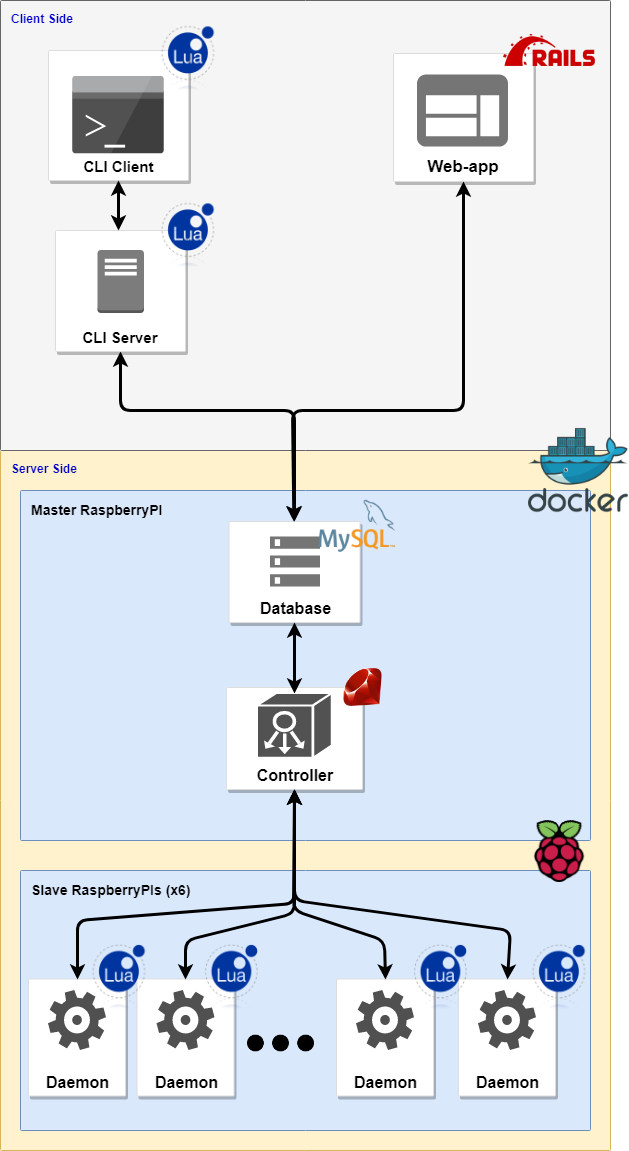
\includegraphics[scale=0.4]{figures/prev_arch.png}
          \caption{\label{prev_arch} Legacy \texttt{Splay} Architecture}
        \end{figure}

        \subsubsection{CLI and Web application}

          Each of these two services were designed to allow interaction
          with the application. These interactions consist of managing the users
          (connection, registration), sending new \texttt{jobs},
          requesting \texttt{logs} and getting informations
          about the application state (number of available nodes, for example).\\

          The CLI service is in fact composed of two sub-services, a server
          ready to receive commands and a client to send commands:
          \begin{itemize}
            \item The CLI server is written in \texttt{Ruby}, running a simple
            \texttt{HTTP} server and waiting for specific \texttt{HTTP} calls containing
            commands representing the wanted interaction (new job, session
            creation, ...).
            \item The CLI client is written in \texttt{Lua} and is composed of
            multiple \texttt{Lua} files, each one representing a command to send
            to the server.
          \end{itemize}

          The web application is written in \texttt{Ruby on Rails}~\cite{ror}, and
          allows the same interactions with the system but through
          a \texttt{HTML} user-interface.\\
          It has thus different \texttt{HTML} pages for user registration, session
          creation, sending jobs and reading logs.\\

          Each of these services communicates with the other components
          through the \textbf{\texttt{databse}}.

        \subsubsection{Database}

          The database is the central communication piece of \texttt{Splay},
          allowing communication between the user and the rest of the
          application.\\
          It contains all the information needed by the different components
          of the application.\\
          The jobs are created by the user applications, then collected by the
          \textbf{\texttt{controller}}.\\

        \subsubsection{Controller}

          The \texttt{controller}, written in \texttt{Ruby}, is the service
          which will orchestrate the job execution sent by the user.\\
          From the job written in the database through the user applications,
          the controller will choose the requested nodes, dispatch the
          algorithm on these nodes, parse the topology if present to make
          use of \texttt{SplayNet} and send to the nodes the different
          informations about network conditions.\\
          This service is also responsible for the \texttt{logs}
          retrieval and creation.

        \subsubsection{Daemons}

          The \textbf{\texttt{daemons}} are the last piece of the system.
          Written in \texttt{Lua}, they are not Linux daemons, but services designed
          to take the role of nodes on which the \texttt{jobs} will
          run. They are also called \textbf{\texttt{Splayds}} in the
          database.\\
          The \texttt{daemons} register on the
          \texttt{controller} through TCP connections so that they
          can communicate.\\

          The creators of \texttt{Splay} made the choice of \texttt{Lua} because it is a very
          small and powerful language, it's tiny core ensuring a light
          footprint, which is conveniant for a scripting language.\\
          Easily embedded with the C language and non-preemptive, it
          facilitates the creation and execution of distributed algorithms.\\

          There is a whole high-level library designed to help the creation of
          distributed algorithms in \texttt{Lua} on \texttt{Splay}, which we
          call \texttt{SplayLib}. This is a rich library that offers for
          example:

          \begin{itemize}
            \item Event management;
            \item RPC servers creation and calls;
            \item High level TCP and UDP servers creation
            \item Global scheduler including a threading system
          \end{itemize}

          The whole manual of this library can be found on the official
          website of Splay~\cite{SplayLib}.


    \section{User Scenarios}

      Before creating a precise list of features to add to \texttt{Splay}, we first
      thought about scenarios. We imagined how someone would want to exercise
      and experiment with his distributed algorithm, using a platform like
      \texttt{Splay}. From these scenarios we would then get the precise new features
      we had to implement in order to make these scenarios possible and
      concrete.\\

      These scenarios are useful to keep track of the progression of our
      work as we would progressively making these a reality, but also useful
      to use them to create tests and ensure these features would be covered.

      \subsection{A student trains on Splay}

        As a student, I would like to be able to put in practice what I learned
        during my courses about distributed systems and applications.\\
        Hopefully, my university provides an existing installation of \texttt{Splay}
        available through the university network.\\
        I can access this service using a web application. After
        registration and login, I have access to a complete \texttt{Lua} Editor that
        allows me to create my own distributed algorithm.\\
        I can also choose parameters such as the number of nodes on
        which run my algorithms, a topology editor to emulate network
        conditions and inject faults.\\
        After I submitted my job, I can get logs about how my algorithm
        performed in the system. I can also choose to kill my job in case
        I did something wrong and the job is not finishing at all.

      \subsection{A professor trains on Splay}

        As a professor, I would like to be able to experiment with a new
        approach of solving the leader election problem among a set of
        nodes.\\
        The new leader election approach is described in a paper with some
        pseudo-code and has special cases of execution when the some nodes
        are linked through extremely slow connections,
        Thanks to \texttt{Splay}, I can rewrite the pseudo-code in actual
        \texttt{Lua} code in a dedicated editor, create special cases of topologies
        thanks to a topology editor.\\
        I can get all the information about the algorithm execution
        thanks to the \texttt{Splay} logging system.

    \section{Cleaning Up and Updating Splay}

      Before starting this thesis, we had the opportunity to get a part-time
      job with the objective of updating the languages and frameworks versions
      used within the project and to get familiar with it. We based our work on
      the latest major release of the application.\\

      We progressively became more familiar with the project, and succeeded
      to upgrades the different versions of the languages and frameworks and
      get back the project state, these versions being:

      \begin{itemize}
        \item \textbf{\texttt{Ruby}}: 1.8.6 $\rightarrow$ 2.5.3
        \item \textbf{\texttt{Lua}}: 5.1 $\rightarrow$ 5.3
        \item \textbf{\texttt{Rails}}: 2.1.0 $\rightarrow$ 5.2.0
      \end{itemize}

      At the end of those ten days of work, we had a healthier and updated
      base to work with and ready to receive the contributions of our thesis.

    \section{Roadmap}

      This section presents our roadmap of the updates and new features
      we wanted to perform on the \texttt{Splay} system. We will first go through
      the changes and updates, and then will talk about the new features.

      \subsection{Changes}

        Between our version update of the \texttt{Splay} components and the
        implementation of new features on the system, a huge amount of
        work had to be achieve. These updates and changes were concerning
        the overall project organization, software quality and maintenance
        guidelines and also a lot of work on the global codebase to fix
        issues and bugs that we noticed during the whole development.
        We will breifly detail each of those changes.

        \subsubsection{Github Organization Recast}

          During the part-time job, we realized that the code organization
          was not really up to current standards and should be changed.\\
          The code of the six different services was located in the same and
          unique repository, this had the consequence of making way harder
          the navigation in the project's tree during the development, the
          clarity of the commits in the Git log and therefore the evolution
          of these different services.\\

          Having to start back from a 2011 commit also made us realize that the
          project was not making use of the git version tagging system, that
          can mark the stable releases of the different versions of the project
          through history, and that we should accomplish this from now on.

        \subsubsection{Testing Implementation}

          The version upgrade process revealed a cruel lack of testing among
          the project, at any level of the application.\\
          The major consequence of this was that we had to make repairs
          step by step because of the languages and frameworks version changes.
          Moreover, we had to base ourselves on a certain global understanding
          of how the project was working and some final execution results of
          scenarios to estimate that the project was functional again.\\

          It was totally impossible to be sure that our changes were not
          impacting some internal behavior of the project in a negative but
          imperceptible way, consequences that were not avoidable in the end
          but that we would only discover thereafter when implementing new
          features.\\
          It was therefore obvious for us that we would have to set up a series
          of tests at different levels of the application during the next
          phases of our work, in order to make the project more maintainable
          than in the state we received it and to ensure that further
          enhancement would be easier to implement.

        \subsubsection{Front-end Refreshment}

          The current full-stack \texttt{Rails} application was quite old and not
          really enjoyable to use for interacting with the \texttt{Splay}
          system. This application was also not following good practices
          promoted by \texttt{Rails} such as REST~\cite{rest} or keeping lightweight
          controllers~\cite{fatmod}.\\
          Therefore, we would need to improve this application in order to
          provide a better user experience and easier way to learn distributed
          algorithm through \texttt{Splay}.

        \subsubsection{Easy installation}

          During our first work on \texttt{Splay}, we noticed that the
          installation and the usage of the system were not easy to handle.\\

          Some services were dockerized, this means that dedicated files
          were present to allow creating images of these services in order
          to run the services in Docker containers.\\
          Containers are "standard units of software that packages up code and
          all its dependencies so the application runs quickly and reliably
          from one computing environment to another. A Docker container image
          is a lightweight, standalone, executable package of software that
          includes everything needed to run an application: code, runtime,
          system tools, system libraries and settings"~\cite{dockercontainer}.\\
          A docker-compose file was present which already facilitated the
          installation. Docker-compose files allows to specify a
          collection of services and links between these services so that
          they will share a common network, allowing easy communication
          between each service~\cite{dockercompose}.\\

          However, these docker images were not perfectly built: healthcheck
          were missing, big and old distribution images were used thus slowing down the
          setup phase and image building.\\
          Also, there was not a proper \textbf{one-click install} script for
          making quick tests.\\
          Therefore, one of our goals was to create clean, small and with
          updated libraries docker images. These images needed to be fully
          integrated between them through the docker-compose file. We should
          provide the users with an automated install script and a running
          script.

      \subsection{New Features}

        In order to reach our goals and be able to provide the users with
        an experience close to the scenarios we imagined, here are the
        features that we needed to add to \texttt{Splay}.

        \subsubsection{Complete Lua editor on the website}

          The first web application of \texttt{Splay} already allowed the user to send
          his own \texttt{Lua} code to create the job but the system was not really
          user-friendly.\\

          As we were going to rebuild the web application and modernize it,
          we wanted to provide the user with a convenient way to prepare
          the job he wanted to send into the \texttt{Splay} system. For that purpose,
          we wanted to integrate an algorithm editor with the following
          characteristics:

          \begin{itemize}
            \item A standalone algorithm editor.
            \item Code coloration for the \texttt{Lua} language in the editor.
            \item An error parsing system so that the user would be warned
            about syntax error in his algorithm.
            \item Optionally some auto-completion features.
          \end{itemize}

          Having this feature available within the job creation page, the user
          could easily and comfortably achieve his tasks on the system.

        \subsubsection{Topology creator/visualization}

          The legacy project managed a definition of a network topology when
          submitting a job. A user could define this topology by setting
          parameters such as:

          \begin{itemize}
            \item Nodes;
            \item Links with latency, bandwidth, packet loss rate and queuing
            length parameters;
            \item Specs with latency, bandwidth, packet loss rate and queuing
            length, that could be used by edges to easily acquire those
            attributes.
          \end{itemize}

          Special nodes like router could also be added to the topology in order
          to create more complex networks. The \texttt{Splay} system will then
          approximate the true parameters for each source-destination by
          emulating this topology.\\

          Following a standard format for topology generators such as
          used in \texttt{ModelNet}~\cite{ModelNet}, \texttt{Splay} users previously
          defined their topologies through sending \texttt{XML} files.\\
          This format not being really user-friendly and quite hard to read,
          and with the fact that format documentation is not easy to find
          on the Internet, we decided that the new web application would have
          to provide an easy way for the user to define his own topology
          still following the standards.\\

          This topology editor should provide a graphical interface with
          allowing an easy configuration. Each change using this interface
          would result in immediate visual feedback thanks to a topology
          visualization tool, such that the user would have a better view about
          his topology than by reading \texttt{XML}. Nevertheless, an \texttt{XML} editor and
          visualization tool should be included in the topology editor which
          would translate the visual output of the tool into readable \texttt{XML} or
          translate its \texttt{XML} content into the visualization tool.\\

          In summary, this tool should provide the user with:

          \begin{itemize}
            \item A topology editor with simple input fields;
            \item A topology visualization tool;
            \item An \texttt{XML} editor;
            \item A way to convert the visual topology in \texttt{XML}, and conversely.
          \end{itemize}

        \subsubsection{Fault Injection}

          The creation of distributed algorithm is a difficult task, and
          moreover, it is hard to make real code that is reliable. The robustness
          and correctness of a distributed solution is the key point to test
          for a designed solution, and manually injecting of fault is painful
          and can take some time as one will need to modify his algorithm.\\

          With the legacy project and the dockerization, it was obviously
          possible to crash a single daemon during the execution of a job, just
          by killing the running container of that daemon.\\
          However, the main problem of this trivial solution is that we cannot
          control where the crash may happen during the code execution, and
          it would require to stop and restart containers. Controlling where
          and when the crash happens is an important feature to explore
          corner cases, solve difficult-to-reproduce bugs.\\
          We wanted to improve this by providing the user with a feature
          allowing him to choose when one or multiple daemons would crash during
          the execution. We came up with two ideas:

          \begin{itemize}
            \item A hard crash in which the node is completely put down
            \item A recovery crash in which the node is relaunched after some
            downtime
          \end{itemize}

          To sum up, our fault injection tool would allow the user to choose
          when (in the execution tree) and where (at one or several nodes) the
          crash happens in the daemon, in an user-friendly way. The best and
          most straightforward way to achieve this is to let
          the user specify those crashpoints in the \texttt{Lua} code within the \texttt{Lua}
          editor.

  \chapter{Architecture and Development}
  \label{chap:dev}

    This chapter will detail our work on the \texttt{Splay} project concerning the
    architectural changes and the modifications of already present features
    of the system we listed in our roadmap.

    \section{Project Analysis and Modifications}

      Having the project in our hands and free to apply changes to achieve our
      goals, we analyzed which parts of the project were problematic today and
      how could we change it to ensure better user experience, better
      maintainability and better overall software quality.

      \subsection{Better User Services}

        The main issue on the architecture of the user services was a code
        duplication issue or at least a duplication related to the solutions
        created to resolve a common problem. The \texttt{Rails} web application and the
        CLI server had the common role of letting the user manipulate the
        database to transmit and gather information to the \textbf{Controller}.\\

        The first decision to make in order to solve this problem was to
        merge those two services into a single one, and to call that new
        service according to his role among the system: The \textbf{Backend},
        according to the viewpoint of the client.\\
        This backend would have the ambition to offer a secured API through
        the usage of \texttt{JWT}~\cite{JWT} (a token based identification system
        for web applications) and therefore allowing the development
        of services around that backend, in our case a web application and
        a command line interface.\\

        The web application would thus use a recent JavaScript technology
        allowing dynamic interactions with the user, and the CLI would use
        a simple and dedicated technology, those two services consuming the
        same API offered by the backend. The backend, for its part, would
        stay in the \texttt{Ruby} ecosystem, in order to keep a technology consistency
        with the global project and the technologies already in use.

      \subsection{Github Repository Reorganization}

        From our analysis on the \texttt{Splay} project, we were not satisfied with how
        it was maintained on Github so far. Our major concerns were the
        following:

        \begin{itemize}
          \item Lack of version tagging to specify stable versions
          \item The code organization was not good and it was hard to
          understand exactly where the different services were located,
          everything was more or less in the same source folder.
        \end{itemize}

        From this analysis, we also realized that the project was really
        lacking documentation in order to help and guide people interested
        in \texttt{Splay} to install and run it.\\

        Therefore, we started with forking the project in a personal repository,
        allowing us to perform complete reorganization of all the directories
        and files composing the project and adding some basic documentation.
        Each service was successfully placed in a distinct directory while
        keeping the docker-compose file working.\\
        The project was cleaner, however, we felt that this was not enough
        and that we could achieve a better structure. The project is big and
        consisting of multiple services interacting with each other but
        not sharing any code. We therefore decided to create a new Github
        organization called \textbf{The Splay Project V2} in which we created
        a distinct repository for each service and one as the main repository
        of the project.\\

        The main repository called \textbf{Splay} contains all the other services
        through the submodule~\cite{GitSubmodules} feature of git. These
        subrepositories representing the new architecture:

        \begin{itemize}
          \item The cli (command line interface);
          \item The daemon (also called \textit{splayd} in the project);
          \item The backend (the merge of the cli\_server and the old web app backend);
          \item The controller;
          \item The new web application (named web\_app).
        \end{itemize}

        Each of these subrepositories is self-sufficient and contains a Dockerfile
        allowing the user to create the related container, to use and test
        the service alone, and therefore also has it's own documentation.\\

        For each master branch of these subrepositories, a link with Dockerhub
        has been made so that each push on master will trigger an automatic build
        of a docker image using the source and uploading it on the
        Dockerhub~\cite{DockerHubGithub}.
        This was specially made to ease the integration testing using a
        continuous integration service, which would have to build every single
        image otherwise.\\

        Now that the services were clearly and logically separated in their
        distinct repositories, it would be really easier for us to track
        the changes made in each service and would ease further improvements
        by \texttt{Splay} maintainers.

    \section{Backend Development}

      In this section, we will go through the development of our new Backend
      as the central communication interface with the database for the user
      applications.\\

      \subsection{The Choice of Rails}

        The controller service and the old pair of services composing the CLI
        having been developed with the \texttt{Ruby} language, and the old web
        application having been developed with \texttt{Ruby on Rails}, it was obvious
        for us to stay within the \texttt{Ruby} ecosystem to create the new service
        that would become what we called the \textbf{Backend}. The technology
        we wanted to use for this development had to offer an efficient
        solution to the following challenges:

        \begin{itemize}
          \item Allowing simple interfacing with the MySQL database in order
          to ensure the communication with the controller, and therefore allow
          the submission of new jobs, the gathering of information about the
          Daemons, etc...
          \item Allow to develop and expose a JSON API allowing other front-end
          services (web application and CLI) to make use of this API and
          interact with the \texttt{Splay} system.
          \item Offer a large choice of libraries for testing, data
          serialization using JSON, and other libraries solving the problems
          we talked about before.
        \end{itemize}

        The both of us already having a certain experience in using \texttt{Ruby on
        Rails}, and for the reasons of ecosystem consistency we talked about
        in the previous sections, we immediately agreed on using this
        framework for the backend.\\
        Staying in the same language ecosystem would allow us to make sure
        that future contributors to the application would not have to master
        too many technologies and therefore make the future evolution
        of \texttt{Splay} easier.\\

        It should also be noticed that, as we exposed it when talking about the
        changes in the renewed software architecture of \texttt{Splay}, the previous
        web application and the CLI server had a similar role although being
        specialized for different applications. However, the common logic
        of these two \texttt{Ruby} services was already present, and a part of the
        work was therefore just a matter of isolating this common logic.\\

        \texttt{Rails} allow to easily develop, besides traditional MVC web
        applications, API-only applications that do not contain all the code
        and complexity needed for presenting \texttt{HTML} views to the user and thus
        having a lighter and more concise codebases.\\

        The ActiveRecord~\cite{activerecord} ORM shipped with the \texttt{Rails}
        applications is also a major advantage for this technology, allowing us
        to easily and efficiently manage the system's jobs and daemons.\\
        Finally, the availability of some libraries such as RSpec~\cite{rspec}
        made for the testing, \texttt{Rubocop}~\cite{Rubocop} for the linter definitely
        made \texttt{Rails} the right technology to choose for the Backend.

      \subsection{Centralization of Splay's Backend}

        One big thing we wanted to achieve was the merge of the old CLI
        server and the backend part from the full-stack old web application
        as those two services were basically achieving the same work and
        holding the same responsibilities.\\

        We started with a fresh \texttt{Ruby on Rails} application, passing the
        generator the \textit{--api} option so that we were provided with
        a clean and simple \texttt{Rails} app without all the front-end dedicated
        files.\\

        Before writing any line of code, the following tools were added
        to the project:

        \begin{itemize}
          \item \textbf{\texttt{Rspec}}: A performant and easy to use \texttt{Ruby} testing
          framework to be able to begin development following the test
          driven development approach.
          \item \textbf{\texttt{Rubocop}}: A static code analyser (linter) to follow
          good codestyle conventions and avoid bad pattern right from the start.
          \item \textbf{\texttt{Travis}}: A continuous integration platform.
          \item \textbf{\texttt{CodeCov}}: A test coverage tool to get further
          information on the test suite.
        \end{itemize}

        Now that the app was ready for development, the major features
        we wanted to provide were the ones provided by the old CLI server and
        were the following:

        \begin{itemize}
          \item User and session management (creation, login)
          \item Job management (creation, deletion, listing, details)
          \item Daemon querying (listing, details)
          \item Job logs querying
        \end{itemize}

        Implementing those features would let us immediately reuse the old
        CLI client for testing purposes and would provide sufficient endpoints
        to start the development of the web application.\\

        \subsubsection{Models}

          The first phase of this centralized backend development was
          to make it hold the responsibility of the database management and
          the way data was handled.\\

          For this purpose, we progressively created database migrations
          for each model of the \texttt{Splay} system (jobs, daemons, users, etc...)
          with the right constraints on their fields.\\
          We reflected these constraints inside the generated \texttt{Rails} models to
          ensure that no corrupted data could be registered into the system,
          having a double check through the application and through the
          database schema.\\
          For each model created, we also wrote model tests to ensure those
          constraints were respected when creating a new model and saving it
          into the database.

        \subsubsection{User Registration}

          To achieve the registration of users, we simply used the
          well-known \texttt{Devise}~\cite{devise} gem (gems are how \texttt{Ruby} libraries are
          called). It provides out-of-the box an efficient and flexible
          authentication solution for \texttt{Rails} applications.\\
          As we were to allow the authentication through a future JSON API,
          the most relevant part in using \texttt{Devise} was to make use of all
          the user registration process given by the gem, using good principles
          in terms of password hashing with salt to store them. We did not
          have to reinvent the wheel about user registration.\\

          Moreover, for any further development or evolution of the application,
          we know that \texttt{Devise} also provides user management modules such as
          Omniauth support, account tracking, registration confirmation
          through emails, and many other listed on the gem webpage.\\

          \texttt{Devise} was therefore the best choice for our registration management,
          even for an API-only \texttt{Rails} application.

        \subsubsection{User Authentication}

          As we mentioned it before, one of the best ways to handle user
          authentication in JSON API applications is by using the JSON Web
          Tokens (\texttt{JWT}), following the industry standard from RFC7519~\cite{rfc7519}.\\

          Upon successful registration or login on the \texttt{Rails} application, a
          \texttt{JWT} is returned to the calling application to provide it with a way
          to authenticate further requests. This \texttt{JWT} holds encrypted
          information (with a secret key) such as the user id to allow the \texttt{Rails}
          app to identify to whothe request belongs. The fact that the token
          is generated in the backend with a secret key also means that the
          token cannot be altered or forged by a malicious application.\\

          To achieve this, we had to syart the work on the API endpoints.
          Before starting to work on those endpoints, we agreed that we would
          follow the principles of REST~\cite{rest} for the API. Endpoints would
          represent entities with classic \texttt{HTTP} verbs to interact with them.\\

          Each endpoint inside our system is managed by the following stack:

          \begin{itemize}
            \item A route entry representing the entity. In this case,
            authentication is linked to the session entity and achieved through
            a POST method, as we want to create a new session.
            \item A controller method corresponding to the endpoint action.
            Here then, a Session controller exists, with a create method in
            which the password checking happens, and where a response is
            returned accordingly.
          \end{itemize}

          As we were in the objective of following good practices, we wanted
          to follow the \textit{"Fat models, skinny controllers"}~\cite{fatski}
          principle.\\
          This principle states that most of the logic should be put in the
          models, and keep the controller with the minimal and relevant logic.
          For example, some methods in the controller require authentication,
          like creating a new job. Therefore, instead of putting all the code
          required to manage that authentication in the controller, it should
          be moved out in a model dedicated to authentication or even in
          the user model.\\

          But instead of bloating our models with the needed inner logic for
          authentication, we created intermediate layers called services~\cite{fatmod}
          in \texttt{Rails}. Those services hold the needed logic to keep the controllers
          nice and clean. In the case of authentication, the controller receives
          the request from the router filled with user data, then delegates
          the task of password verification, token generation if successful,
          and just return the result in the response. The same process was also
          applied to manage registration through the API, as it needed the \texttt{JWT}
          layer to be in a working state.

        \subsubsection{Splay Endpoints}

          From all the previous tasks on the backend, we now had all the
          necessary basis to create the other endpoints in order to let
          an authenticated user interact with \texttt{Splay}.\\

          Once again, we created an authentication service that checks
          the request's token to verify whether or not the user was valid or
          if he had the necessary rights to perform the requested action.\\

          The endpoints we created are the following:

          \begin{table}[H]
            \centering
            \begin{tabular}{|l|l|}
            \hline
            \textbf{Endpoint} & \textbf{Methods}       \\ \hline
            Users             & Create, destroy, index \\
            Sessions          & Create                 \\
            Splayds           & Index                  \\
            Jobs              & Index, show            \\
            Logs              & Show                   \\ \hline
            \end{tabular}
          \end{table}

          The \textsc{create} methods required additional checks in corresponding
          services, to carefully create the entity in the database with
          the data sent with the request and make sure those data were
          satisfying the constraints.\\

        \subsubsection{Error Handling}

          In order to provide the best response to the applications
          communicating with the backend anf follow the REST
          principles, we wanted to respond with the right \texttt{HTTP} status code in
          case of errors.\\

          A successful request is answered with a 200
          status code by the \texttt{Rails} application by default.\\
          \texttt{Rails} has a really convenient way to raise errors and catch them
          in the same or upper component on the call stack. We used that tool
          to implement the following error management strategy:

          \begin{itemize}
            \item Each Controller of our API inherits from a common file
            called \textit{ApplicationController}
            \item This ApplicationController holds a set of catchers (rescue
            in the \texttt{Ruby} language) to catch which errors happen in our
            application:
              \begin{itemize}
                \item The entity that the user wants to create isn not valid,
                this means he sent bad parameters through the request;
                \item The requested action is not authorized for this user;
                \item The request is malformed (missing fields or badly forged
                request);
                \item The requested entity does not exist (for example a user
                wants to get the job details for a non-existing job)
              \end{itemize}
            \item Then, in any controller or service used by a controller, we
            can raise an error and associate an error message, which will be
            automatically catch at the root level and trigger a response with
            the right \texttt{HTTP} status code and the given error message.
          \end{itemize}

    \section{Web Application Development}

      This section will detail the development of the new web application,
      starting with the choice of technology, and then going through the
      development details.

      \subsection{Choosing the Framework}

        As we made the decision that the web application would only be a
        front-end application making use of a centralized backend offering
        a complete JSON API, we wanted to use a front-end web development
        framework that would satisfy the following conditions: \\

        \begin{itemize}
          \item Light in terms of weightness;
          \item Ease of development and maintenance;
          \item Access to numerous third-party libraries;
          \item Popular enough to ensure support over time.
        \end{itemize}

        In order to develop a front-end application, the \texttt{JavaScript} ecosystem
        was an obvious choice, and we made a pre-selection among the most
        popular web framework on the market and recognized for their qualities:
        \texttt{ReactJS}, \texttt{Angular} and \texttt{VueJS}.\\
        We rapidly removed Angular from our list because we preferred the
        component-based UI development offered by the two other frameworks,
        which were lighter and avoided having to develop in the MVC style.
        Even if we both had previous experience with \texttt{ReactJS} thanks to a
        Cloud Computing course at UCLouvain, we decided to go for \texttt{Vue}
        instead of React.\\

        The first major advantage of \texttt{Vue} is how light it is. We also took into
        account the fact that this technology was gaining in popularity for
        multiple years now to be today a huge player in the world of web
        technologies. Moreover, as we took some time to develop a proof
        of concept application using \texttt{Vue}, we were totally satisfied with the
        simplicity of development that that framework was offering to the
        developers.\\
        \texttt{Vue} allowed us to be totally confident into the fact
        that going for this technology would allow any further contributor
        of the \texttt{Splay} project to easily get in and participate to the
        development.\\
        Indeed, a \texttt{Vue} application is organized around single components, each
        having its own \texttt{HTML} template, their \texttt{CSS} style declarations and
        the associated \texttt{JavaScript} code. No other exotic language is required.\\
        The fact that the framework belongs to the \texttt{JavaScript} ecosystem and is
        associated to the NPM package manager also allows to take advantage of
        numerous existing libraries, such as data visualization libraries,
        testing libraries, etc...\\

        For all those reasons, \texttt{Vue} was the best choice for a
        web application and also allowing us to develop with something
        we liked and with recent technologies, besides providing an efficient
        solution to the conditions we needed for the technology.

      \subsection{The new front-end application development}

        As the development of the backend was started, we started in the
        meantime the development of a Single Page Application using
        the \texttt{Vue} framework.\\

        After removing the old files of the previous web application, we
        created a basic \texttt{Vue} project (version 2.5.X at that time) having a
        simple home page and using the \texttt{bootstrap-vue} package~\cite{BootstrapVue}.
        \textbf{Bootstrap}~\cite{Bootstrap} is a
        well-known \texttt{HTML}, \texttt{CSS} and \texttt{JavaScript} framework used to create responsive
        and modern web interface.\\
        Bootstrap is a real Swiss-army knife among the design framework
        and helped us building a visually pleasant and easy to use
        web application with minimal custom \texttt{CSS} and \texttt{JavaScript} code.\\

        The next step was to build a register and a login page to allow
        user management. In order to manage different pages in the same \texttt{Vue}
        project, we installed the \texttt{Vue-Router} package, a \texttt{Vue} extension
        allowing the navigation through different URI within the same
        single page application (without any reload and additional requests
        to the web server).\\
        This package allows the user to switch from page to page
        as he was on a regular website. Those pages being in fact components
        loaded depending on the selected URI in a root component.\\
        We then created the associated routes for the user registration and
        connection, the forms directly using the freshly written API available
        on the backend.\\
        In order to use that JSON API and allow communications with the
        backend, we used \texttt{axios}~\cite{axios}, a popular \texttt{HTTP} Javascript client.
        This being done, our web application allowed the user to create its
        account and connect to it, receiving an authentication token that
        was stored on the client browser to allow auto-login on the next
        visits.\\

        In order to get the same features as the legacy web application,
        we created a \textbf{monitoring} page (showed on
        figure~\ref{monitor_web}), on which important
        information would be displayed to the user in lists:

        \begin{itemize}
          \item A list of \texttt{Splay} daemons (created by the controller) is retrieved
          from the backend and displayed with global information in a nice
          bootstrap table.
          \item A second table used for \texttt{jobs} (also fetched from the backend) is also
          displayed with general data about these jobs.
        \end{itemize}

        \begin{figure}
          \centering
          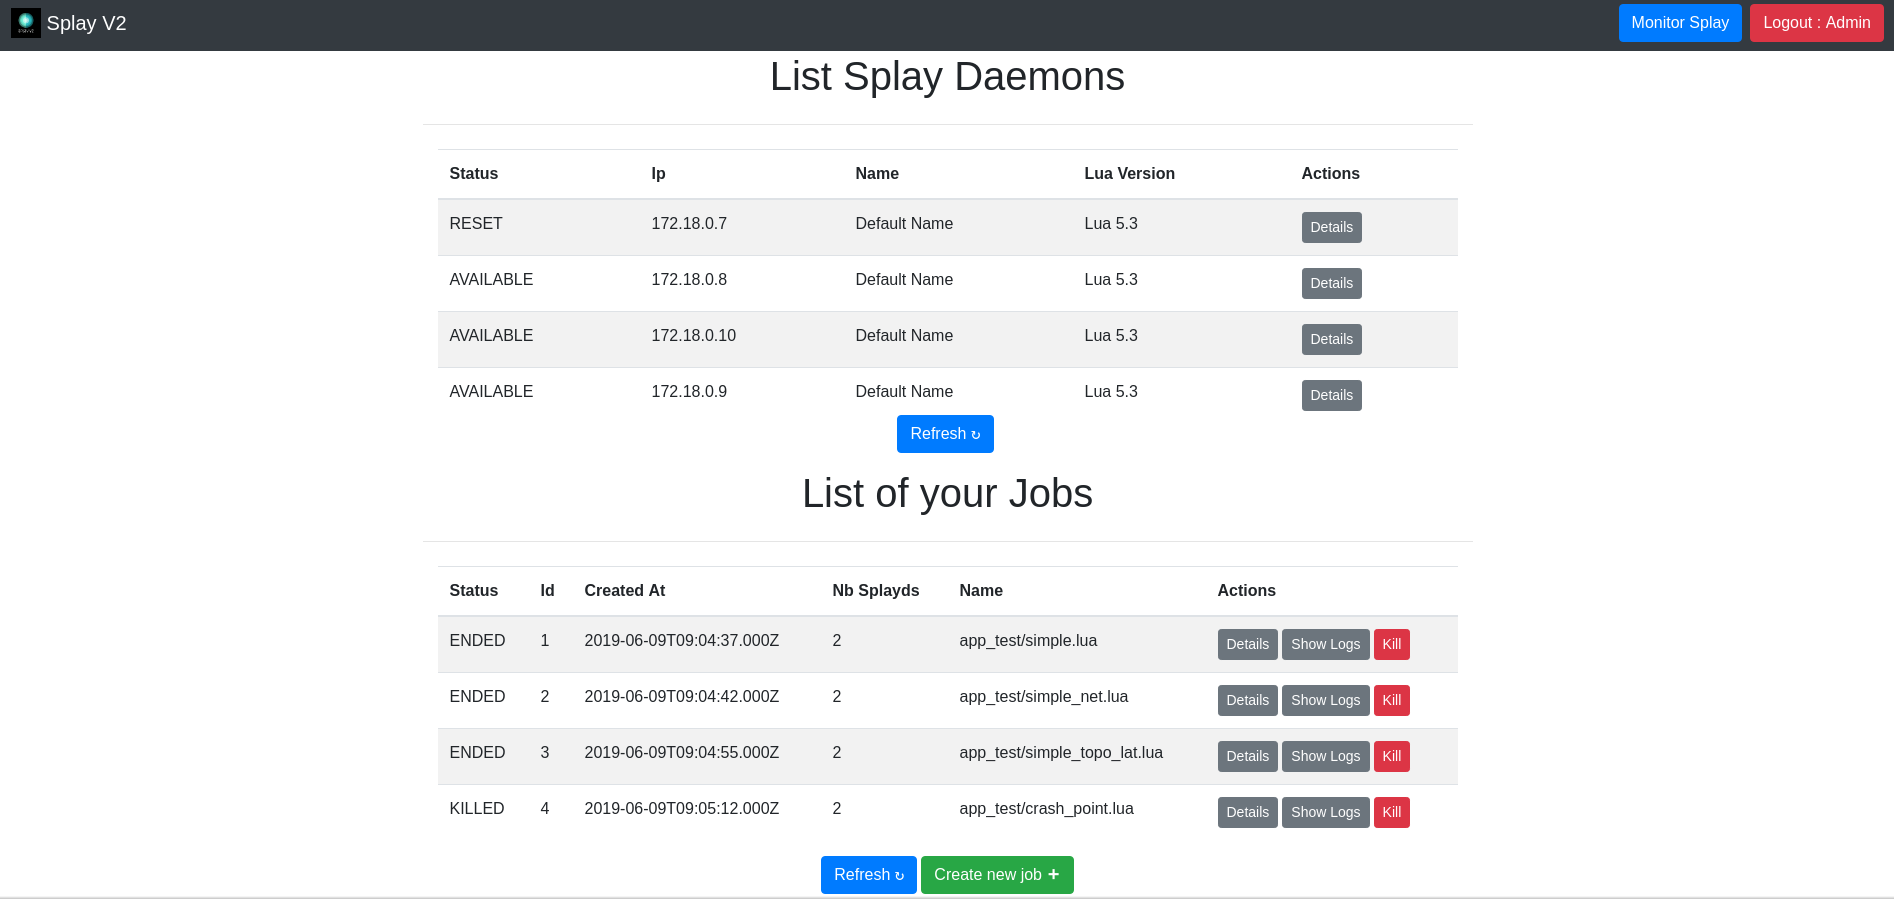
\includegraphics[scale=0.27]{figures/monitor.png}
          \caption{\label{monitor_web} Monitoring Page}
        \end{figure}

        The user can choose to
        get more details about a specific \texttt{Splay} daemon or job using a button
        on the application, the result is showed in
        figures~\ref{daemon_details}~and~\ref{job_details}. He can also choose
        to kill a job, sending the related command to the backend to let the
        controller achieve that job killing.

        \begin{figure}
          \centering
          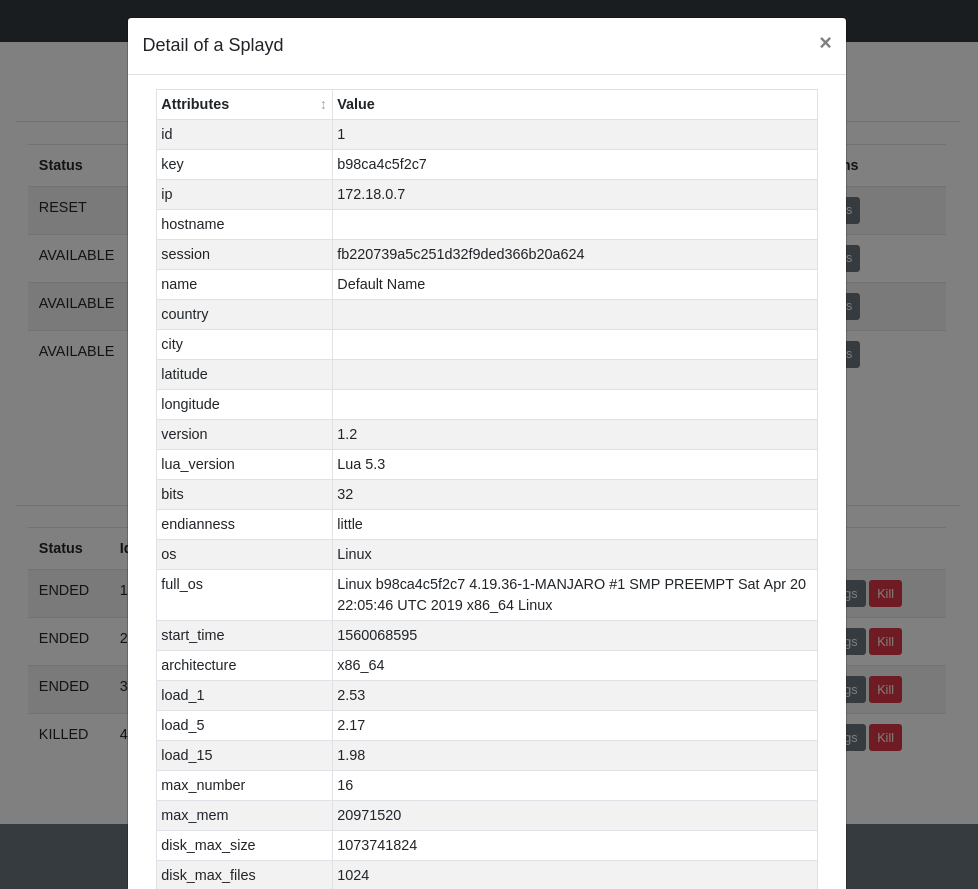
\includegraphics[scale=0.55]{figures/daemondetails.png}
          \caption{\label{daemon_details} Daemon Details}
        \end{figure}

        \begin{figure}
          \centering
          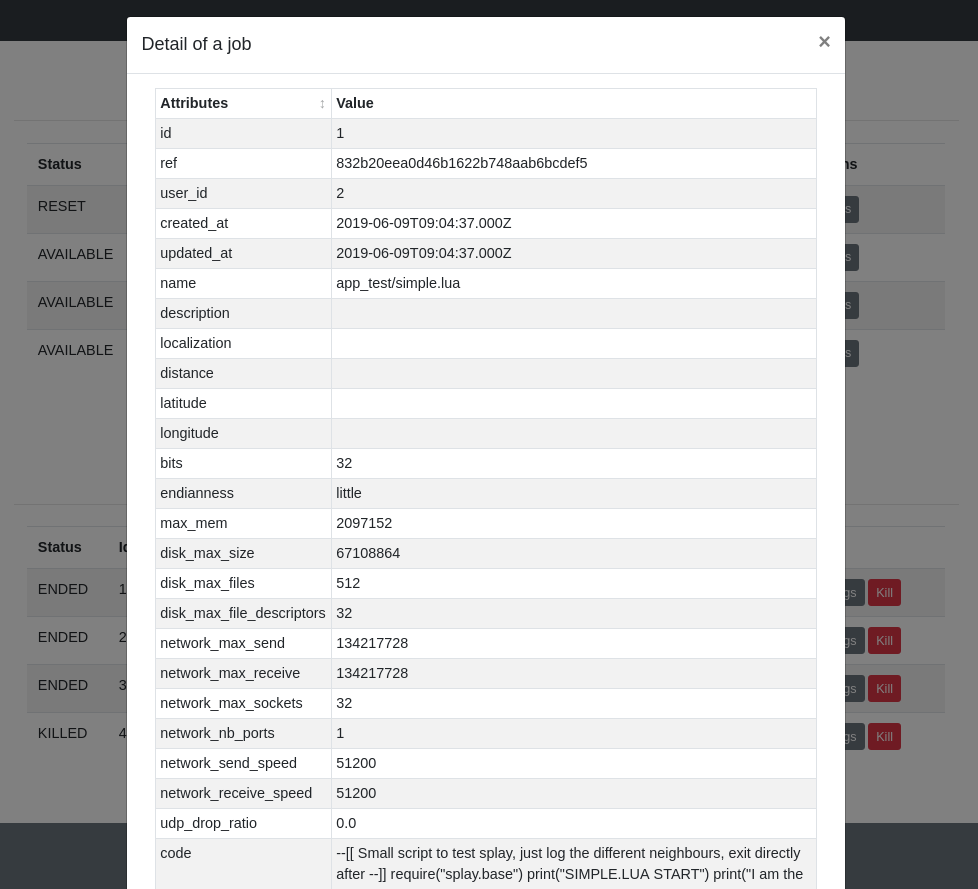
\includegraphics[scale=0.55]{figures/jobdetails.png}
          \caption{\label{job_details} Job Details}
        \end{figure}

        The creation of a job is done through a simple form. We implemented
        an automatic check of the fields using the \texttt{vee-validate}
        package~\cite{VeeValidate}. As the data sent to the backend is also
        checked before using those to create a new job, \texttt{vee-validate} offers us
        a double validation and allows giving the user better feedback
        about any field he would have forgotten or wrongly filled.\\
        \texttt{Vee-validate} is a small package solving the problem of
        manual checking of forms by adding some properties to inputs, and it
        makes our code more compact and less messy.\\

        This being done, we almost retrieved all the legacy features (for the
        web application) but in a much nicer way, with a modern solution
        and maintainable code. Only the log downloading functionality was
        missing at this point. \\
        As soon as we completed the backend with the logging endpoint, we
        add this feature to the website with some improvements. When the
        job is running or is finished, the user can see the log (using a
        button next to the job details) which holds the involved daemons logs
        with, for each line, the time and the daemon id indication. The user
        can then choose to download the logs as a textfile (as it was possible
        before) and check how his job performed.

    \section{CLI Development}

      This section will detail the CLI application development, starting
      with an explanation of why we chose a precise technology to achieve
      this application, then detailing how we implemented it on the system.

      \subsection{Using Python}

        The old pair of services intended to compose the CLI service were
        written in \texttt{Lua} on the client side, and the CLI server was in \texttt{Ruby}. As
        the server's logic would be moved and merged into the \textbf{Backend}
        service, and as we wanted to keep a command line interface application
        in order to run tests of the global project, we needed to reevaluate
        the relevance of \texttt{Lua} for this application.\\

        It is more than probable that \texttt{Lua} was used for coherence reasons back
        in the days, and to avoid scattering \texttt{Splay} around too many different
        technologies (although \texttt{Ruby} may have been used too instead of \texttt{Lua}).
        Still, maybe today this choice was not the most relevant for a CLI
        application. Indeed, our small client CLI had to:

        \begin{itemize}
          \item Be simple;
          \item Be concise;
          \item Be written in an easy-to-use language;
          \item Having convenient libraries allowing to create simple CLI apps.
        \end{itemize}

        However, we inherited of an application scattered in multiples \texttt{Lua}
        files, each file representing a CLI command. We therefore had code
        duplication, as each file was repeating the process of parsing the user
        arguments when the program was called, and also repeating the process
        of reaching the server through a \texttt{HTTP} library in \texttt{Lua}.\\
        \texttt{Ruby} was indeed a relevant option if we wanted to restrict the number
        of different technologies in use among the project, but \texttt{Python} was
        a better choice to write such a simple script as our CLI. \texttt{Python} has
        a lot of very convenient libraries to treat \texttt{HTTP} calls and to
        manage and parse user arguments when creating a CLI application.

      \subsection{Developing the CLI}

        A nice CLI client was still needed within the project, whether it
        would be for quick testing from people experienced with using the
        \texttt{Splay} application and wanting to have small scripts making their
        work faster, for the developers in order to allow easy manual testing
        of the \texttt{Splay} endpoints or, and most importantly, to allow automatic
        feature testing and continuous integration (this would still be
        possible using the web application but would require a lot more
        configuration to handle a headless browser, making the test suite
        too much complicated).\\

        We started by creating a simple \texttt{Python} script executable
        through Bash and running version 3 of \texttt{Python}.\\

        The first step was to set up the available commands to create our CLI.
        In order to make the code the cleanest and simplest possible, we
        decided to use the \texttt{Click}~\cite{click} library, a perfect
        \texttt{Python} package designed to create powerful CLI's with just a little
        code.\\
        The steps for creating a command are:

        \begin{itemize}
          \item Declaring the creation of a command;
          \item Declaring eventual arguments and constraints on those arguments;
          \item Declaring eventual options for the command;
          \item Writing the body of the related command.
        \end{itemize}

        Each command or option can be supplemented with help messages. Then
        \texttt{Click} reassembles all of this and format theoutput of the CLI,
        displaying to the user help details if requested and even help details
        for specific commands.\\

        The next step was to make real use of the Backend's API, thus we used
        \texttt{requests}~\cite{requests} and \textbf{json} \texttt{Python}'s libraries to
        achieve the \texttt{HTTP} communication and the JSON requests encoding and
        responses parsing.\\

        This complete rewrite of the CLI allowed us to remove thousands of
        \texttt{Lua} lines of code and to obtain two hundred of simple and
        maintainable lines \texttt{Python} lines of code achieving the same features.

    \section{Bug fix on Daemon and Controller}

      The daemon and controller are the only services
      among \texttt{Splay} that were not assigned a complete refactor because of how
      complex and long that task would have been. Nevertheless, these services
      were not stable enough and a lot of bugs were found during our tests.\\
      We therefore needed to apply a lot of corrective changes on those, and
      this section details this.

      \subsection{Controller changes}

        Most of the issues on the controller were due to a previous
        maintainers misuse of the sequel calls (a \texttt{Ruby} library offering a MySQL
        toolkit), but this is an overall list of all the changes that we
        applied:

        \begin{itemize}
          \item \textbf{Sequel Calls}: We have detected that in the legacy
          source code, a maintainer wanted to change and replace the old library
          called \texttt{dbd-mysql}~\cite{dbdMysql} for the \texttt{Sequel}~\cite{Sequel} one. We
          totally agreed with this as \texttt{dbd-mysql} has not been not updated since
          2010 and still has bugs whereas Sequel manages different type of
          rmdb's and is still an active project.\\
          The problem was that most of the \texttt{SQL} calls through Sequel were wrongly
          written, therefore a lot of calls were returning no data at all or
          inserting nothing. We thus had to check every Sequel usage in all the
          code and change for the right call. We also tried in the same process
          to clean as much as possible the raw \texttt{SQL} string calls by using
          interpolation (see the improvements section in the conclusion).
          \item \textbf{Communication with daemons}: The communication between daemons
          and the controller was not consistent is some cases. For example, the
          logs retrieval was buggy because daemons were sending more
          information than expected by the controller.\\
          Therefore, logs retrial and creation were fixed, but
          also improved to be cleaner and more readable (previously an issue on
          the old project~\cite{logTimestamps}).
          \item \textbf{Small Changes}: We added more logs when needed and
          removed the unneeded ones, the database creation responsibility has
          been delegated to the backend (previously held by the controller). We
          also used \texttt{Rubocop}~\cite{Rubocop} in order to get a uniformized code
          style and correct wrong patterns in the code.
        \end{itemize}

      \subsection{Daemons changes}

        We had to change and fix small parts of the daemon in order to make
        it consistent with the controller (concerning the communication part)
        and also made some improvements on the \texttt{Splay}'s \texttt{Lua} library.

        \begin{itemize}
          \item As explained in the controller part, we fixed the communication
          protocol used between the daemon and the controller, mainly for
          the logging and the registration of daemons on the controller.
          \item The topology socket restriction is now automatically achieved
          when a topology is given with a job. This restriction is used to
          simulate the topology settings, limiting the bandwidth and creating
          latency.\\
          The topology socket has a major issue in its design, the restriction
          is only based on the ip and port, therefore if a daemon uses a client
          port (tcp or udp), the server will answer respond to an unknown port
          without any restriction.\\
          To bypass this, we created a new topology restriction only based on
          the ip, but that means that all the nodes (daemons) need to have a
          different ip (thanks to docker, this is the case), but that is
          something that should be improved and changed and we will talk about
          it in the improvements section.
          \item We removed the \texttt{LuaCrypto} library from the daemon and added
          luaossl to replace it. The main reason of this change was that
          \texttt{LuaCrypto} cannot use the last Linux's OpenSSL package (due to a
          security issue, and older versions cannot be used in newer OS),
          \texttt{LuaCrypto} was also not updated anymore and moreover, an issue about
          this was open in the old project repository~\cite{sslLib}.\\
          We therefore updated the code to make use of the new luaossl library.
          \item Multiple bug fixes mainly due to the \texttt{Lua} version change needed
          to be solved.
        \end{itemize}

    \section{Software Architectures}

      Here is an overview of the previous architecture and the renewed one,
      so that the reader can have a better and more visual understanding
      of the changes we made and talked about in the previous sections.

      \begin{figure}[!tbp]
        \centering
        \begin{subfigure}{0.45\textwidth}
          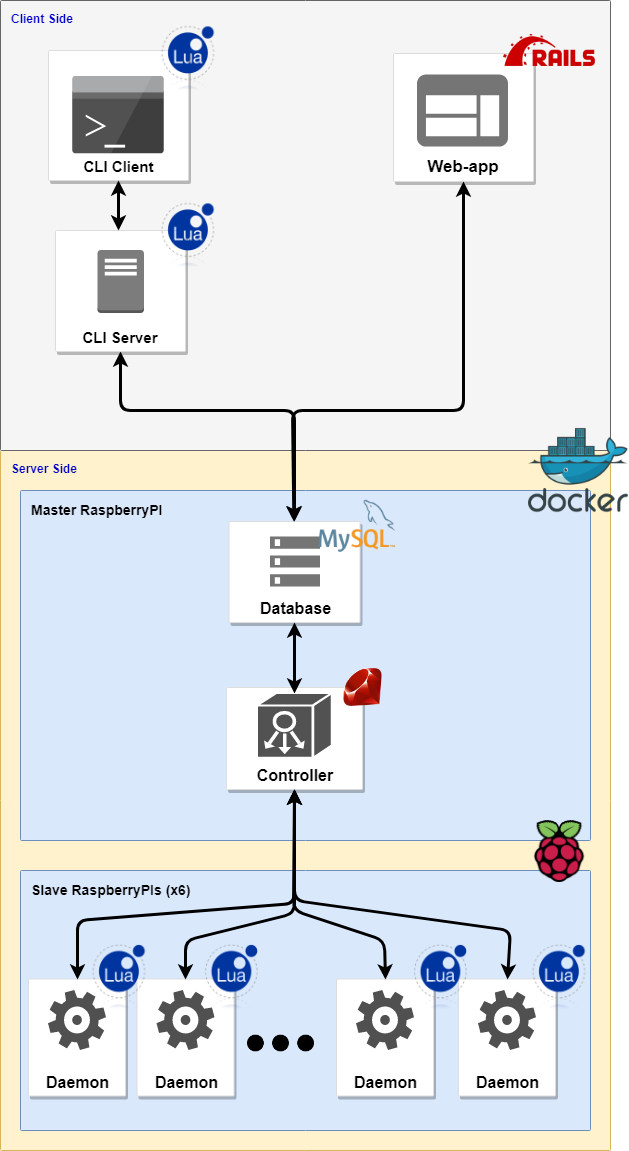
\includegraphics[width=\textwidth]{figures/prev_arch.png}
          \caption{Previous Architecture}
        \end{subfigure}
        \hfill
        \begin{subfigure}{0.45\textwidth}
          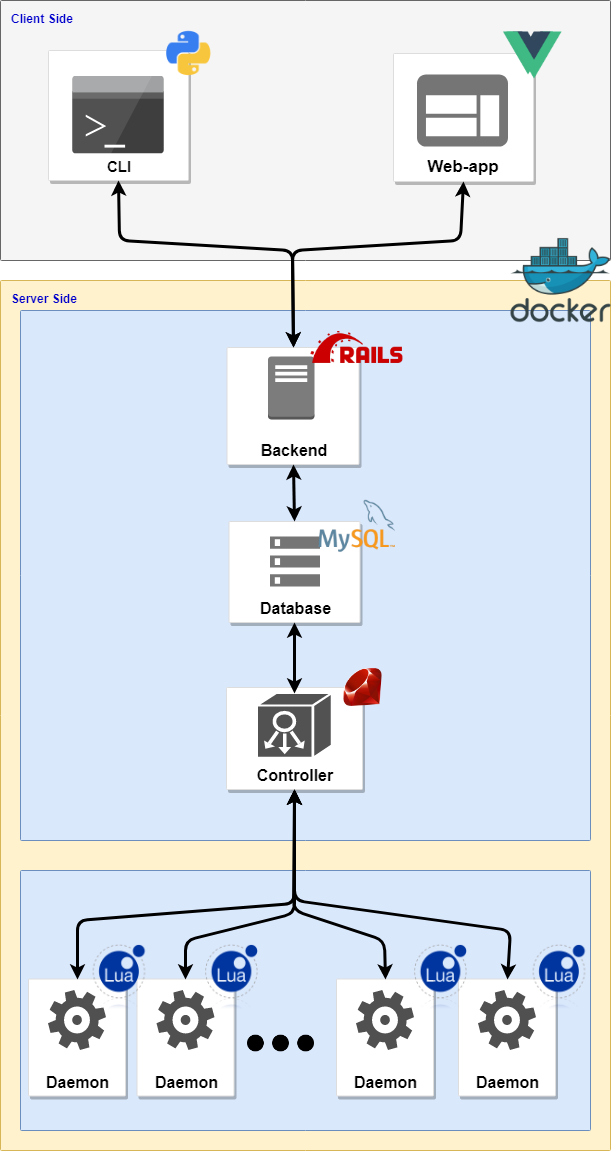
\includegraphics[width=\textwidth]{figures/new_arch.png}
          \caption{Renewed Architecture}
        \end{subfigure}
        \caption{Splay Architectural Comparison}
        \label{fig:test}
      \end{figure}

  \chapter{Quality Assurance}
  \label{chap:qual}

    In this chapter, we will talk about the techniques we used to ensure the
    quality of the code. We put the effort into ensuring quality into two
    parts, one being the way we organized ourselves to work together on \texttt{Splay},
    the other being testing and validation on the codebase.

    \section{Development Methodology}

      Being two students on this development project necessarily required a
      method of organizing ourselves more effective than for a development
      project alone.\\

      Thanks to the courses about AGILE methodologies we followed during our
      studies, and both of us have had the occasion of acquiring
      experience in a professional environment through internships and part-time jobs,
      we wanted to put to work this knowledge and good practices acquired in
      the project management domain.

        \subsection{Kanban}

          The first tool we put in place, and this from the very beginning of
          the update period of \texttt{Splay}, was a Kanban using the online website
          Trello~\cite{trello}. The kanban allowed us to: \\

          \begin{itemize}
            \item Have a clear and precise view of the remaining tasks we had
            to achieve in the backlog, and also about the development state of
            all the other tasks.
            \item Encourage and even oblige ourselves to translate the features
            we had to implement into sufficiently detailed and explicit cards on
            the kanban. This process has the benefit of refining or making
            features the most explicit possible before starting the development.
            \item Have a way of tracking the project's progression and offering
            to all the people related to the project a simple and effective way
            to keep themselves informed about \texttt{Splay}'s state.
            \item To focus ourselves on specific tasks and to work in an
            iterative and efficient way.
          \end{itemize}

        \subsection{Testing and Validation}

          We wanted to integrate testing and
          validation processes as part of our development methodology and
          therefore followed a test-driven development approach.\\
          The tests and quality were thus not only a validation technique to
          apply on to work afterward, but a complete part of the development
          and helping us to reach our goals.

        \subsection{Github and Gitflow}

          The project and all the services composing it are versioned using the
          \textit{Git} versioning system and are hosted on the online service
          \textit{Github}.\\
          We, therefore, organized our work on the \texttt{Gitflow} model. Each feature or
          task we created on the kanban was meant to receive its very own
          branch, starting from the main branch.
          Once the feature finished and tested, a pull request was made asking
          to merge the feature branch to the main branch.\\
          The first benefit of this was obviously to keep the main branch in
          a working state with healthy and finished features. Indeed, as
          we will explain in the following section, we set up a series of tools
          to allow ensuring a branch was passing the tests before allowing any
          merge on the master branch.\\

          \begin{figure}[H]
            \centering
            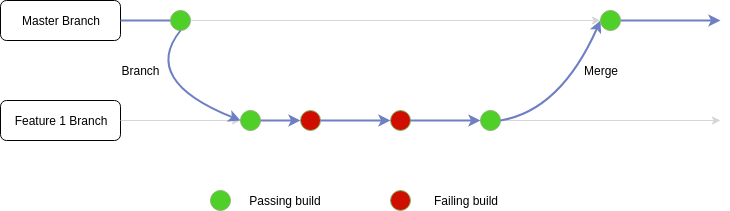
\includegraphics[scale=0.6]{figures/gitflow.png}
            \caption{\label{gitworkflow} Gitflow Workflow}
          \end{figure}

          The second benefit of this methodology was to
          permit code reviews, once again towards the goal of ensuring quality.
          Each time one of us was done with the development of a
          task and was issuing a pull request, the other was assigned as code
          reviewer and was in charge of making this code review, accepting the
          pull request and doing the merge, or to detect errors or bugs as the
          outcome of the code review and therefore to ask for changes to the
          pull request issuer.\\

          Besides the main code review's benefit of reducing the number of
          errors or bugs, this process also allowed each of us to keep ourselves
          aware and keep ourselves up to date with all the different changes
          happening on the different services. Indeed, it was impossible for
          us to work together on every single service, because
          of the number of services and inter-dependant features we had to
          develop.

    \section{Testing and Validation}

      In this section, we talk more deeply about the way we wanted to ensure
      the testing and the validation part in the \texttt{Splay} project, whether it be
      at the global system level or at the user functionalities level. Each
      section will go through the different services and how we tested then, and
      also how we tested the application globally.\\

      The fact that \texttt{Splay} had only few tests (not directly integrated) in the state we receive it
      motivated us into developing a solid test suite for the system.
      Indeed, that fact made our task much harder because we were progressing
      in the dark, each minor change was prone to create dysfunctions that we
      might only notice way later during our work.\\

      The test writing phase took place from the very beginning of our work on
      \texttt{Splay} as part of our development methodology,
      to make sure that we were ensuring the new code's maintainability, but
      also to progressively give \texttt{Splay}'s core new tests to have a healthy
      and maintainable final product.\\

      The figure~\ref{global_testing} details the whole \texttt{Splay} project with the different
      test suites and procedures. Each of them will be detailed in this chapter.

      \begin{figure}[H]
        \centering
        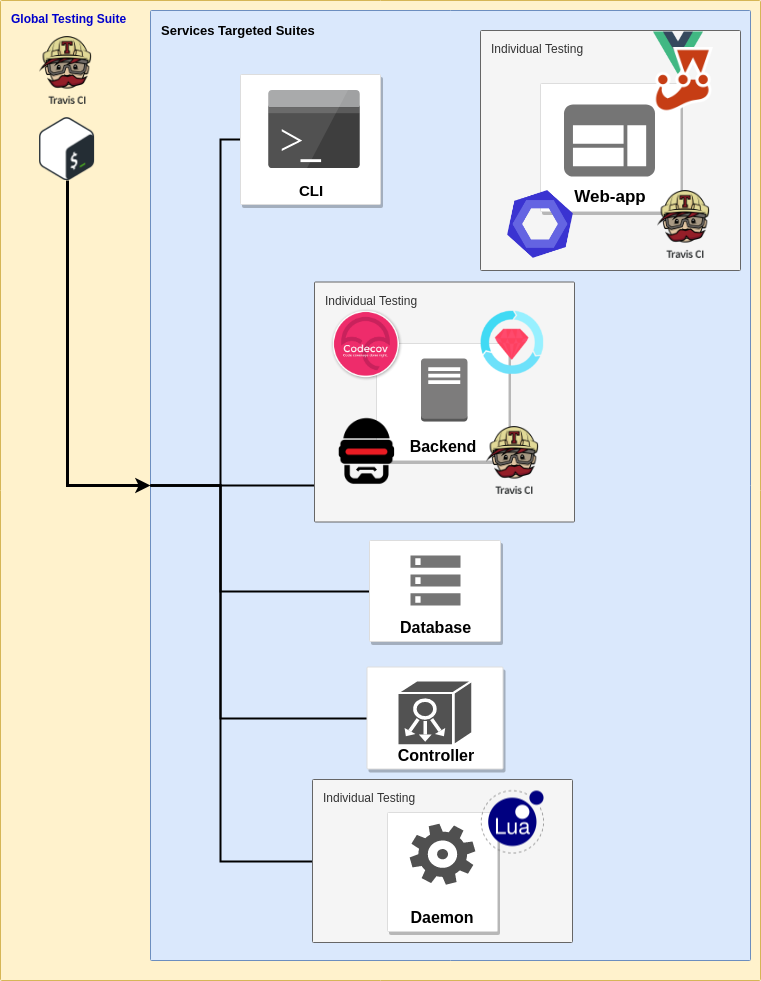
\includegraphics[scale=0.55]{figures/global_testing.png}
        \caption{\label{global_testing} Global Testing in Splay}
      \end{figure}

      \subsection{Testing in Web App}

        As we chose \texttt{Vue} as our framework for the web application service,
        all we had to deal with was components. As \texttt{Vue} is organized around
        the use of components, the immediate reward of this was that we would
        be able to write tests dedicated to isolated and simple components.

        \subsubsection{Jest}

          In order to test the components composing the application, we
          went for the \texttt{Jest}~\cite{jest} testing framework, which was advised
          as unit testing framework during the project creation.\\

          Testing JavaScript is not always the simplest thing to achieve, the
          ecosystem being in constant evolution with diverse solutions emerging
          trying to fit with the evolution and the apparition of a lot of
          other JavaScript frameworks.\\
          But Jest was a really good pick as the testing framework, as it was
          developed by Facebook and designed to fit with the majority of the
          most used front-end framework and this with almost no configuration and
          providing us with a really simple API.\\

          In order to test the application using \texttt{Jest}, we created a directories
          hierarchy reflecting the \texttt{Vue} components hierarchy we created, thus
          a test file corresponding to a component file. In each of these
          test specifications, we decided to target the core part of each
          component: the methods.\\
          Indeed, there is no need to test whether or not a click on a button
          triggers the associated action as this is part of the \texttt{Vue} system. What
          we wanted to test was the triggered action we wrote ourselves and
          were simply functions.\\
          Each file, therefore, tests that the related components can be
          successfully instantiated within the application, then runs a series
          of \textbf{unit tests} validating the expected behavior of methods.

        \subsubsection{ESLint}

          Provided by default when creating a new \texttt{Vue} project, ESLint~\cite{eslint}
          is a JavaScript linter that allows the developer to
          make sure he is not writing code inducing problematic patterns or not
          respecting code guidelines.\\
          This helps to keep a consistent code style as we were two developers working
          on this project and increase the overall code quality and
          maintainability. We chose not to change any preset of the shipped-in
          ESLint configuration to ensure following common guidelines among the \texttt{Vue}
          community and make sure any developer joining the \texttt{Splay} project will
          be able to work on the web application seamlessly.

      \subsection{Testing in Backend}

        As a reminder, the Backend has the following
        roles:

        \begin{itemize}
          \item It has the responsibility of handling the database and
          defining its structure.
          \item It must offer a JSON API allowing other applications to interact
          with the system.
        \end{itemize}

        The backend is written in \texttt{Rails}, therefore, we have access to the
        ActiveRecord ORM which allows manipulating the database by associating
        tables to models. These models are thus granted with attributes,
        constraints to comply with on these attributes following the constraints
        listed in the database schema, but also granted with methods. This data
        modelization allows us to do model testing.

        The backend role being only to offer a JSON API to the different client
        services through an authentication system using JSON Web tokens, a
        request testing suite should be implemented to validate our set of
        endpoints and the mechanism of authentication.
        The data responses being sent to the calling applications in the form
        of JSON responses, we had to serialize our models and therefore this
        part was also subject to testing.

        \subsubsection{RSpec}

          \texttt{RSpec}~\cite{rspec} is a library aiming to ease behavior Driven
          Development on \texttt{Ruby} projects. BDD and TDD (Test-Driven Development) are
          practices we wanted to follow for our work on the \texttt{Splay} development,
          this would allow us to adopt a green-red-refactor work cycle but also
          to focus on writing natural language scenarios and then translating
          them into test scenarios.

        \subsubsection{Model Testing}

          As we made it explicit in upper sections, the \texttt{Rails} ORM layer offers
          a reflexion about the database constraints by representing its
          tables under the form of models granted with attributes, that we can
          enrich with additional attributes, methods and an overlay of
          additional validations (such as validations on attributes
          combinations, or more complex constraints between the models).\\

          Hence, this additional abstraction needs to be covered with a
          sufficient validation set, which we did by applying
          \textbf{Model Testing}. This overlay applied to the
          models but also the basic constraints specified in the database's
          schema.\\

          Therefore, this testing set is offering a double validation on the
          database field constraints, but also validations on the business
          logic we added in the application.

        \subsubsection{Request Testing}

          The request tests inside the Backend service are the most important
          tests we wrote in terms of code coverage, but also, it covers almost
          every implemented features inside of this \texttt{Splay} service.\\

          The request specs among the RSpec tool are made to simulate
          the behavior of a third-party application sending a request to
          our service and therefore making the whole \texttt{Rails} stack runs
          to provide an answer to this request.\\
          Each request is going through the following elements:

          \begin{figure}[H]
            \centering
            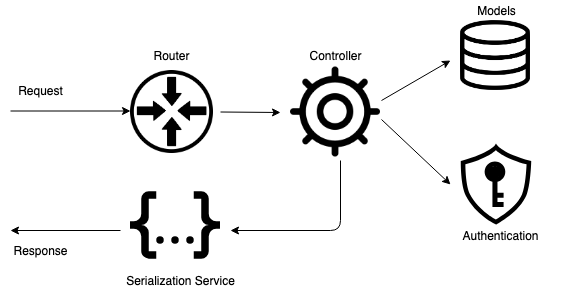
\includegraphics[scale=0.6]{figures/request_test.png}
            \caption{\label{request_test} Request Lifetime in Backend Service}
          \end{figure}

          Each route of the application is tested, exploring different possible
          scenarios for the incoming request (the identification token provided
          is invalid, the token is valid but the requested action is not
          authorized for the associated user). At the end, we have a testing set
          that exercises the entire application, simply by sending a request and
          making expectations about the awaited response from the application.

        \subsubsection{Code Coverage - Simple Cov}

          We chose to use Simple Cov in succession of the testing applied to
          the Backend. This tool allows us to measure the code coverage of \texttt{Ruby}
          application and to provide the developer with useful information
          thanks to its test execution analysis.\\

          Our ambition on the user part of the \texttt{Splay} project was a total recast of
          the services in more simple and maintainable ones, it was therefore
          obvious and simple for us to reach a total coverage of that new codebase
          with a test suite and thus chose to use that tool.\\

          The benefits we found in using a code coverage tool were the
          following:

          \begin{itemize}
            \item Encourage the TDD approach, as it's easier and better to
            write the tests covering the feature and then writing the feature
            instead of writing the feature and then tests in order to reach
            the coverage level
            \item Ensuring we do not let parts of the code or certain branches
            in conditional statements being untested
            \item Refrain to write useless code. The tests are supposed to cover
            which features should exist, a decrease in the coverage level
            might then spot bad patterns or code being outside the scope
            of the feature.
          \end{itemize}

        \subsubsection{Code Quality - Rubocop}

          We used \texttt{Rubocop} as the last piece of the tool stack designed to ensure
          the code quality within the service. \texttt{Rubocop} is a static code analysis
          tool (linter) allowing to detect violations to a set of rules about
          the code style and good practices (too many lines of code for a method,
          too many variables instantiations, too many conditional branching
          in the code, ...).

      \subsection{Testing in Daemons}

        The Daemon is a critical part of the project as it has to communicate
        with the controller to receive the jobs, run the jobs and return
        information to the controller about the job state. But the Daemon also
        provides a rich distributed library (\texttt{Splay} lib) written in \texttt{Lua} to the user.\\
        In the legacy project, only a few tests were present and their
        task was to check the installation and to test some very basic features
        (small functionalities) of the \texttt{Lua} \texttt{Splay} library. Some of those tests
        were not passing anymore (if they did pass one day), and no testing
        library was used.\\

        We wanted to change this, so we started by adding a testing library
        called Busted~\cite{busted}. This library allowed elegant unit testing,
        still under active development and fully integrated with \texttt{Lua} 5.3.\\
        Then we successfully transformed the old existing tests into busted
        tests. With only this single change, we were able to detect some
        anomalies in the lib code and fix these. We added some test steps
        in the docker image creation to avoid creating malformed images.\\

        Moreover, we added a lot of tests about each modification we made
        (openssl package updated, new misc functions, small changes in existing
        functions, ...) and also about the new features.\\
        Sadly the whole \texttt{Splay} lib of the Daemon is not entirely tested,
        the huge amount of code (some being documented and some not) made it
        really hard for us to make it ourselves during the period of this
        thesis. But our work on the Daemon is still improving the maintainability
        for future improvement or refactoring.

      \subsection{Integration Testing}

        In order to automatically test the project as a whole, we also wanted to
        develop a functional test suite. This test suite would be relatively
        simple but complete enough to make sure that we could test the developed
        features in a global way among the system and to achieve this goal we
        just had to translate our user scenarios into test scenarios.\\

        For these functional tests, we did not use complex technology and
        thought that a Bash scripts series would be more than sufficient to
        reach our goal. Bash scripts could indeed not allow us to recreate user
        behavior using \texttt{Splay} through the web application, but as this
        application is using the exact same API offered by the Backend than the
        CLI application, we could simulate user behavior through that CLI (and
        that is one of the reasons why we decided to keep a CLI application
        within the project).\\

        The integration tests were placed in a dedicated directory at the \texttt{Splay}
        project's root, and execute the following actions for each test:

        \begin{itemize}
          \item Cleaning the containers.
          \item Rebuilding the different services listed in the docker-compose
          file.
          \item Starting up the services.
          \item Executing commands through the CLI.
          \item Checking the returned response sent by the CLI and displaying
          whether the test phase has succeeded or failed in the terminal.
        \end{itemize}

        By proceeding this way and with the fact of using our user scenarios to
        determine the actions described in the test suite, we can make sure
        that the implementation of our features is functional and will stay
        functional through the lifetime and evolutions of \texttt{Splay}. Moreover, those
        tests are adding an additional validation layer compared to the tests
        targeting the different services individually. We have here tests that
        are involving each service in concrete scenarios and reflecting real
        working conditions of the project, and also testing interactions
        between the services.

      \subsection{Continuous Integration}

        Once again in a way to ensure quality, the different services were placed
        on the Travis CI~\cite{travis} continuous integration platform. Travis
        can be coupled with Github to detect any change on the branches and
        automatically run a test procedure listed in a script and then offer
        feedback on how the test suite went.\\

        \texttt{Splay} being an open source project, that we hope to see growing in the
        future, its collaborative development will inevitably happen through
        the Github organization in which the different repositories are located.\\
        The coupling of Travis with Github allows, in the case of a pull request,
        to gather the review about the test execution on the branch asking to be
        merged with the main branch, and therefore to make sure the build is
        clean and the tests are passing before merging the new code, as
        explained before in the \texttt{Gitflow} section.

    \chapter{New Features}
    \label{chap:newfeat}

      In the previous chapters, we went through the development of all
      the changes we had to implement in the already existing features
      and the software architecture of the project, and also explained
      in details how we ensured quality insurance among the whole project,
      we now explain the development of the new features we implemented in
      \texttt{Splay}.

      \section{Web Application enhancement}

        The new web application implemented in \texttt{Vue}, which we detailed in
        the previous chapters, has received some of our important new features
        of the project aiming to provide a better user experience: the
        integrated algorithm editor and the topology creation tool.

        \subsection{The Lua editor}

          One of our objectives for the web application was to provide the user
          with a fully integrated \texttt{Lua} editor within the application and
          available during the job creation process.\\
          The idea of entirely building ourselves this editor was quickly
          moved aside, as it would take too much time to achieve and would not
          be a solution allowing easy evolution through time.\\
          We then found a great package named \texttt{Brace}, a browserified
          version of the Ace editor~\cite{Ace}. Ace can handle hundreds of
          different programming languages concerning syntax coloration,
          error handling, line number displaying.\\

          The integration of Ace in the project was really easy and light thanks
          to the available npm package. The editor now displays \texttt{Lua} code
          perfectly colorized and highlights syntax errors.\\

          Sadly, no built-in auto-completion module was available from the
          Brace package. It would have been possible for us to add our own
          auto-complete script in the Ace editor, but that was a too long
          task to achieve for the time we had, we thus decided to move on and
          keep the result as it was.\\

          The resulting editor can be seen in figure~\ref{luaeditor}.

          \begin{figure}
            \centering
            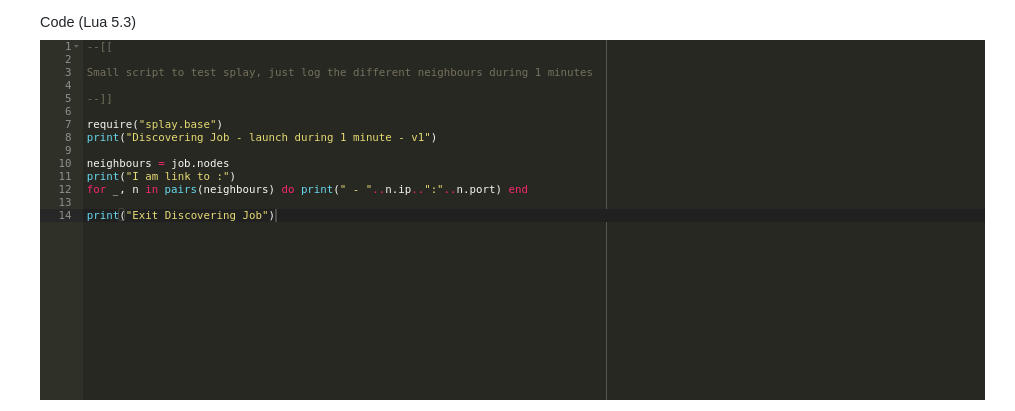
\includegraphics[scale=0.55]{figures/luaeditor.png}
            \caption{\label{luaeditor} Lua Editor}
          \end{figure}

      \subsection{Topology creation}

        The second objective concerning the web application was to provide to the
        user an easy way to enter the topology details, where the distributed algorithm
        will run into. The previous and only way to send a topology
        to the server was to write a whole \texttt{XML} file following the ModelNet
        topology representation, a somehow tedious and error-prone process.\\

        The first step in our solution was to create a user interface with
        form fields for each of the components of the topology:

        \begin{itemize}
          \item \textbf{Nodes}: Virtual nodes or gateways.
          \item \textbf{Specs}: Set of predefined settings such as the
          bandwidth and packet loss rate which would then be used by
          a link.
          \item \textbf{Links}: Linking two nodes, choosing a spec to
          inherit its settings and maybe overriding one of the spec settings
          with its own.
        \end{itemize}

        \begin{figure}[H]
          \centering
          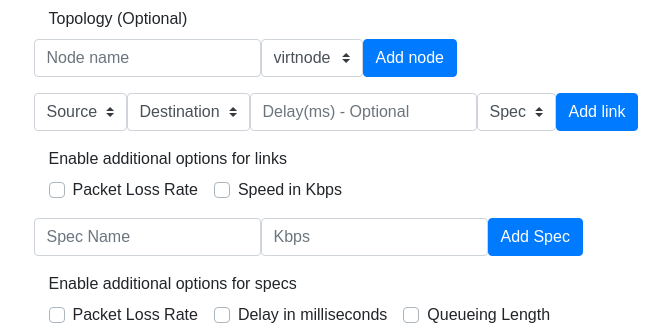
\includegraphics[scale=0.6]{figures/editor_topology.png}
          \caption{\label{editor_topology} UI Topology Editor}
        \end{figure}

        We have set validations behind the scenes and
        prevent the user from creating wrong settings such as a link having the
        same node as source and destination and ensure the topology would
        fit in the \texttt{Splay} system. To help a user manage the created
        elements of a topology, a simple summary of these elements are
        output on the page with the related information. A simple click on those
        allows to delete the corresponding element from the topology.\\
        Indeed, any deletion of a node would delete the link it is associated
        to, or any deletion of a spec would delete the associated links.\\

        \begin{figure}[H]
          \centering
          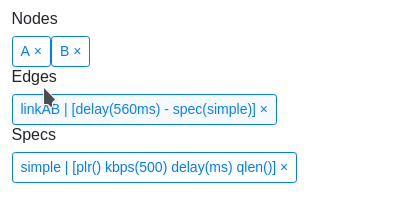
\includegraphics[scale=0.6]{figures/recap_topology.png}
          \caption{\label{recap_topology} Interactive Recap of the topology}
        \end{figure}

        To help the user get a better visualization of his topology, we
        decided to implement a network visualization solution using the
        Cytoscape \texttt{cytoscape} library.\\
        On any update from the form explained above, the change is reflected
        inside our network visualization component adding the new links or
        nodes created by the user so that he can keep track of his topology
        evolution in a more pleasant way.\\

        \begin{figure}[H]
          \centering
          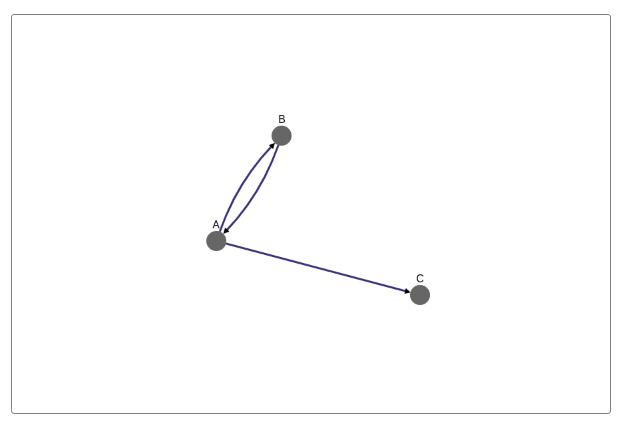
\includegraphics[scale=0.6]{figures/visual_topology.png}
          \caption{\label{visual_topology} visualization of the topology}
        \end{figure}

        Once the user is done editing his topology, he does not have to
        do anything more. We created the editor so that the saved entities
        of it (being JSON elements) would be directly transformed into the
        corresponding \texttt{XML} file and sent to the backend alongside the
        job.\\

        However, using a visual tool with buttons and inputs is not always
        the fastest and most practical thing for someone more experienced. We
        thought that some \texttt{Splay} users would probably not want to be obliged
        to play with our topology editor and would keep their topology
        settings in some file alongside with their code.\\
        Therefore, We wanted to allow the user to play with \texttt{XML} directly
        if he wanted to, offering the following service:

        \begin{itemize}
          \item A user creating the topology could also translate what's
          displayed in the visual editor into the \texttt{XML} definition.
          \item A user creating the topology could directly paste
          his \texttt{XML} topology in some editor and also have the option of
          translating it into a visualization.
        \end{itemize}

        Addressing these two issues was an extremely easy task, the job of
        converting the topology in \texttt{XML} was already available and done on
        the job submission. We reused the Brace package used
        for the \texttt{Lua} code editor to create an \texttt{XML} Topology editor.\\
        The user could then trigger an \texttt{XML} creation into the Brace editor
        before sending the job or paste its code into the Brace editor, and
        then ask for reflecting the \texttt{XML} topology into the visual editor. It
        was just then the matter of parsing the XML and generating the
        corresponding JSON entities, reusing the functions we already wrote
        for the \texttt{Vue} components composing this global feature.

        \begin{figure}[H]
          \centering
          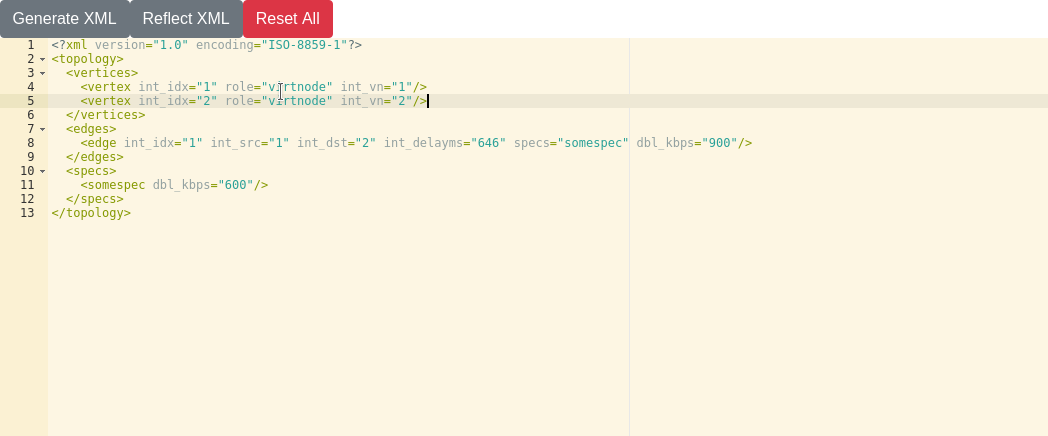
\includegraphics[scale=0.5]{figures/xml_topology.png}
          \caption{\label{xml_topology} XML Display and Editor}
        \end{figure}

    \section{Fault injection}

      The fault injection feature (or crash point) is achieved on the daemon
      side of the application. Indeed, we wanted to be able to trigger a crash
      of the code in the middle of the execution tree, therefore only the
      daemon was able to handle with precision the crash.\\

      We therefore made the decision to use a domain specific language (DSL)
      for the crash management so that a user could define the crash point
      in the \texttt{Lua} code as a comment. During the job execution phase, just before
      executing the user code, we parse the code and gather those crash
      points generate crashes.

      \subsection{Domain Specific Language (DSL)}

        We defined our small domain specific language to be simple to use
        for the user and flexible enough for the parsing phase. This DSL
        needed to be integrated into the \texttt{Lua} code without forcing the user to
        modify its algorithm code and trying to avoid totally crashing
        the daemon in case of the crash points specified by the user were
        not correct.\\
        Also, the difference in terms of th number of lines of code between the
        source code before and after the parsing needed to be the same in
        order to keep the feedback error messages right (getting the same line
        number when locating the error).\\

        For these reasons, we designed the feature so that a crash point has
        to be represented as \textbf{one line} of code and beginning by
        two hyphens (--) which indicates a \texttt{Lua} comment.\\
        To avoid interpreting any other comment, those crash points must
        contain the keyword \textsc{CRASH POINT}. Achieving this by comments
        was probably the best option so that the real code does not get any
        interference with our crash point functionality. The crash then
        happens exactly where the crash point is defined, it is, therefore,
        possible to make the execution code crashing anywhere (thread, middle
        of a function, etc...)\\

        Secondly, a fault is defined by a type, the moment it should occur and
        on which node it should occur. These characteristics also needed to
        be specified within our DSL. Each characteristic follows the
        \textsc{CRASH POINT} keyword and are separated by a colon, their are
        defined by their keyword and values if needed.

        \begin{itemize}
          \item First, the chosen nodes to be affected by the crash must be
          specified. For this purpose, the user must add the ids of the
          affected nodes separated by a space (ids begin at 1 -> number of
          daemons used).
          \item The type of crash can be specified by its name and optional
          parameters
          \item The moment where the crash occurs
        \end{itemize}

        Our final DSL looks like this:

        \begin{lstlisting}[style=MyBash]
-- CRASH POINT id_splayd [id_splayd [...]]: <TYPE>: <WHEN>
<TYPE> => STOP | RECOVERY <float>
<WHEN> => AFTER <int> | RANDOM <float>
        \end{lstlisting}

        We defined two types of crash and two ways to
        define the moment of the crash.\\
        A stop crash means that the node will die forever. Conversely, a
        recovery crash means that the node will crash and recover after the
        number of seconds specified by the user (float number).\\
        Concerning the moment of the crash, there are two possible specification:

        \begin{itemize}
          \item The \textbf{AFTER} keyword means that the user specifies the
          number of loops to achieve before the crash occurs. For example,
          the value 5 at the beginning of the loop means that this loop will
          execute 5 times before triggering the crash, whereas 0 triggers
          an immediate crash.
          \item The \textbf{RANDOM} keyword means that the user specifies a
          probability between 0 and 1 that the node crashes each time it
          encounters the crash point through the code execution. For example,
          if the user specified 1, the crash will occur at first execution
          (similar to AFTER 0).
        \end{itemize}

        To summarize the DSL, we created some positive examples (crash definition valid) :

        \begin{lstlisting}[style=MyLua]
-- Crash forever the node 1 and 2 at the 4th passage
-- in the code
-- CRASH POINT 1 2: STOP: AFTER    3

-- At each time that the code (node 1) pass by this comment,
-- there is 0.0002 chance to crash the node 1
--CRASH POINT 1: STOP: RANDOM 0.0002

-- Crash immediately when the comment is encouter in
-- the node 1, but this node will recover after 2 sec
-- CRASH POINT 1: RECOVERY 2: AFTER 0

-- Have 50 % probability to crash at each pass for
-- the node 1, 2, 3, 4, 5. But recover immediately
-- CRASH POINT 1 2 3 4 5:RECOVERY 0:RANDOM 0.5
          \end{lstlisting}

        We also added some negative examples (will not trigger any crash
        and will not crash the daemon):

        \begin{lstlisting}[style=MyLua]
-- will not work because Crash point not in uppercase
--Crash Point 1 2: STOP: AFTER 3

-- will not work because no node is specified.
-- CRASH POINT:RECOVERY  965:   AFTER 3

-- will not work because RECOVER is not a valid
-- type (but warning expected).
-- CRASH POINT 1 2:RECOVER 1: AFTER 3

-- will not work because TIME is not a valid type
-- for now (but error expected).
-- CRASH POINT 1 2:RECOVERY 1: TIME 3
        \end{lstlisting}

      \subsection{Parsing}

        The code parsing phase is achieved just before that the user code
        is effectively launched on each node (daemon). The parsing will
        create a table with information about each crash point found in the
        user code and which nodes this crash should occur on.\\
        This table is then saved in a library called \textit{"splay.crash"},
        and is used by the nodes to get the crash information using an id
        number which will retrieve the corresponding crash information.\\

        The parsing phase actually assigns to the nodes a new code where the
        crash point comments specified by the user are transformed and
        replaced (if no error is found) by a function call containing the
        crash id number. Therefore, when the code executes, the crash
        function will access the library and will act depending on what
        information is stored into the crash table (the type of crash and
        the triggering moment).

        The parsing handles any error the user could have done about the
        syntax of the crash point.\\
        Parsing is done line by line and if any error is found (also error
        about the parsing code itself), the concerned line will be unchanged, and
        a warning or error message will be written in the logs.\\
        This feature is fully written in Lua using the basic regex matcher of Lua
        \cite{RegexLua} (it is not a complete Regex implementation).

      \subsection{Execution}

        We saw how exactly we defined our DSL and how we achieve the parsing,
        we shall now see in detail how the crashes exactly happen, how they
        are handled and how the nodes recover if they have to.\\

        The Lua multithreading is non-preemptive, this means that we cannot stop a thread from the
        outside~\cite{CoroutineLua}. This particularity helps to simplify distributed algorithms,
        but for the fault injection, it limits the field of possibility
        (we cannot kill a thread without killing the process).
        Then, a solution is to exit the process it-self by using an OS function (os.exit),
        then kill all threads. We also have the possibility of sending an exit
        status code to the process (as parameters of the function),
        which is very convenient for knowing if we need to restart or stay
        down after a crash point was triggered.\\

        With this way of exiting, we can create artificial crash points which
        will immediately kill every coroutine (threads) of Lua and its
        current execution. Moreover, we can pass special exit status codes
        in order to send messages to the parent process.\\
        In order to use these exit codes, we created a fork (available from
        the C splay library) before parsing the crash point and executing
        the user code.\\
        Therefore, the child process will execute the parsing of the crash
        point and proceed to the code execution, and the parent process will
        wait to receive the exit status code of its child. We added a Lua
        function (waitpid) for this purpose and used the original waitpid
        of C \cite{waitpid}.\\

        When the child process terminates (either in a normal way or because
        of a crash), the parent process checks the exit status code and act
        accordingly. If the exit status code is 65 or 66, it means that a
        crash has been triggered (or that the user wants to exit
        with one of these values). We choosed to use 65 and 66 because
        according to this article~\cite{StatusCode}, the range is 64-113
        is proposed to be user-defined status code.

        \begin{itemize}
          \item \textbf{65}: Means a STOP crash, no restart is needed
          \item \textbf{66}: Means a RECOVERY crash
        \end{itemize}

        The recovery crash is then achieved recursively, the parent process
        creating another fork, and the crash table is reset when reparsing
        the original code. Moreover, when it is a recovery crash, the user
        can define the downtime. Our simple solution to achieve this is by
        using the non-preemptive feature of Lua and forcing the process
        to sleep x seconds without any yield coroutine (therefore other
        coroutines cannot execute any code) before crashing.

  \chapter{Use Case}
  \label{chap:usercase}

    We will take the example of a student following a course on distributed
    applications and distributed systems who wants to prototype the Raft
    leader election algorithm on five different nodes. He choses to use
    \texttt{Splay} for his tests using his own laptop (or if available, a cluster
    of mini-computers) and right now he has no available installation of the
    \texttt{Splay} system. We are going to describe the different steps that our
    student will go through by using the \texttt{Splay} application.\\

    First, he needs to install a \texttt{Splay} environment on his own computer. Then,
    with the help of the \texttt{Splay} library, he will build a basic Raft leader
    election implementation.\\
    Following this, he would like to understand what is happening during the
    execution of Raft by showing an animation of the evolution of the
    endpoints states.\\
    Moreover, he would like to test its algorithm implementation through
    different network topologies and analyse the solution
    robustness by injecting faults at key parts of the algorithm.

    \section{Installation of Splay}

      The student only has his laptop to work on his distributed algorithms
      courses, and hopefully, he found out on the \texttt{Splay}'s main Github
      repository~\cite{SplayV2Git} that the installation does not depend on
      any operating system or hardware. The README file of the Github project
      precisely describes how to install \texttt{Splay}. Then, following the
      instructions, he clones the main repository and installs docker and
      docker-compose on his computer.\\
      In order to run \texttt{Splay} on production mode, he runs the following
      commands: \\

      \begin{lstlisting}[style=MyBash]
docker-compose -f docker-compose.prod.yml up -d web_app controller
# 7 daemons because it is recommended to have more than needed
docker-compose -f docker-compose.prod.yml up -d --scale daemon=7
      \end{lstlisting}

      The images are downloaded from prebuilt images (from dockerhub) for
      each service, some little wait time is requested for this download
      phase and for each service to start.\\
      Once this is done, the student has access to the web application of
      the \texttt{Splay} system, using his favorite web browser with this url:
      \url{http://localhost:8080/}.\\
      He creates his own account by registering on the platform, opens a new
      session (which will be kept open for the next time he wants to use
      the system). He can now easily prototype his first distributed job.

    \section{Implementation of Raft in Lua}

      After the successful easy installation, the real work can start, our
      student will create his own implementation of Raft using the \texttt{Splay}
      library.

      \subsection{Raft election}

        Raft is a consensus algorithm, often used as an alternative as Paxos because
        it seems more understandable. The problem of consensus is fundamental
        in fault-tolerant distributed system, it involves the agreements of
        a value by multiple instances. When a desicion is validated by the system,
        it is final. Typically a consensus algorithm make progress only if there is
        a majority of node alive and with a connection between them, it is
        also the case of Raft. \\

        Raft works in two phases: a leader election phase and a phase of
        value replication initiated by client to the current leader.\\
        During leader election phase, where a unique leader is elected
        through a voting process. To remain the leader, the node holding
        this position sends hearbeats to avoid that other nodes trigger a
        new election. A leader election can be triggered by any node if it
        does not receives heartbeats during a certain period of time (election
        timeout).\\
        This election timeout is randomly chosen between two values
        to avoid a much as possible any conflit of election. When a node
        triggers an election, it becomes a candidate and request votes to
        the other nodes, and becomes leader if it receives a majority of votes.\\
        Also, on each election a term (number increasing monotonically)
        is used to progress the election.\\
        We will present and focus only on this election subproblem of
        Raft, because the state machine replication heavily increases the complexity and
        the readability (even in Lua).\\

        The Raft implementation that we will present in the next subsection is based on
        some papers~\cite{RaftPaper} and articles/courses~\cite{RaftSlide}~\cite{RaftSite}.
        We have implemented the Lua code of the Raft consensus leader
        election part with the help of the \texttt{Splay} lib~\cite{SplayLib}.
        \texttt{Splay} lib supplies a great number of tool to communicate
        between nodes, we chose to use Remote Procedure Call (RPC) over UDP.\\

      \subsection{Creation of the Algorithm}

        The student finally created the Lua version of the Raft leader
        election subproblem, which is not trivial, but made
        understandable. We cut the commented code in multiple parts to improved the readability,
        the whole code can be found on the github repository
        \footnote{\url{https://github.com/splay-project-v2/cli/blob/master/app_test/raft_election.lua}}.

        \begin{minipage}{\linewidth}
        \begin{lstlisting}[style=MySmallLua,caption={Initialisation}]
require("splay.base")
local json = require("json")
local urpc = require("splay.urpc")

-- Overwrite the print to show the job position (node index)
do
	local p = print
	print = function(...)
		p(job.position.." : "..(...))
	end
end

majority_threshold = #job.nodes / 2
thread_heartbeat = nil

volatile_state = {
    state = "follower", -- follower, candidate or leader
}

-- Save in stable storage (here just a file)
persistent_state = {
    current_term = 0,
    voted_for = nil,
}

-- Timeout for each purpose in second
election_timeout = 1.5 -- random: [election_timeout, 2 * election_timeout]
rpc_timeout = 0.5
heartbeat_timeout = 0.6

-- Timeout variable (to check if timeout has been canceled)
election_time = nil

-- File to save the persistent state
filename_persistent = "pers"..job.ref..".json"
local pers_file = io.open(filename_persistent, "r")
if pers_file ~= nil then
    persistent_state = json.decode(pers_file:read("*a"))
    pers_file:close()
end
        \end{lstlisting}
        \end{minipage}

        \begin{minipage}{\linewidth}
        \begin{lstlisting}[style=MySmallLua,caption={Utils functions for all nodes}]
function save_persistent_state()
    pers_file = io.open(filename_persistent, "w+")
    pers_file:write(json.encode(persistent_state))
    pers_file:close()
end

-- If someone have a bigger term -> stepdown (request or response)
function stepdown(term)
    print("Stepdown : "..term.." > "..persistent_state.current_term)
    persistent_state.current_term = tonumber(term)
    persistent_state.voted_for = nil
    save_persistent_state()
    volatile_state.state = "follower"
    set_election_timeout()

    -- If I was leader but obviously not anymore - remove pediodic heartbeat
    if thread_heartbeat ~= nil then
        events.kill(thread_heartbeat)
    end
end

local inc = 0
function uprc_call_timeout(node, data, timeout)
    inc = inc + 1 -- Unique name for each rpc
    local name = "urpc.call:"..inc
    local ok = false
    local term, res = nil, false
    local function call()
        term, res = urpc.call(node, data, timeout*10)
        ok = true
        events.fire(name)
    end
    local function timeout_rec()
        events.thread(function()
            events.sleep(timeout)
            if (ok == false) then
                call()
                timeout_rec()
            end
        end)
    end
    call()
    timeout_rec()
    events.wait(name, timeout*10) -- After 9 retry stop anyway -> return nil, false
    return term, res
end

function send_vote_request(node, node_index)
    print("Send vote request to node "..json.encode(node_index))

    local term, vote_granted = uprc_call_timeout(node, {
        "request_vote", persistent_state.current_term, job.position
    }, rpc_timeout)
    return term, vote_granted
end

function send_append_entry(node_index, node, entry)
    print("Send append entry ("..json.encode(entry)..") to node "..node_index)

    local term, success = uprc_call_timeout(node, {
        "append_entry", persistent_state.current_term, job.position, entry
    }, rpc_timeout)
    return term, success
end
        \end{lstlisting}
        \end{minipage}


        \begin{minipage}{\linewidth}
        \begin{lstlisting}[style=MySmallLua,caption={Utils functions for the leader only}]
function heartbeat()
    for i, n in pairs(job.nodes) do
        if i ~= job.position then
            events.thread(function ()
                term, success = send_append_entry(i, n, nil)
                if term ~= nil and term > persistent_state.current_term then
                    stepdown(term)
                end
            end)
        end
    end
end

function become_leader()
    print("I Become the LEADER !")
    volatile_state.state = "leader"
    -- cancelled timout election
    election_time = misc.time()
    -- trigger the heartbeart directly and periodically
    heartbeat()
    thread_heartbeat = events.periodic(heartbeat_timeout, function() heartbeat() end)
    -- No client simulation for now (because no replication log)
end
        \end{lstlisting}
        \end{minipage}

        \begin{minipage}{\linewidth}
        \begin{lstlisting}[style=MySmallLua,caption={RPC functions}]
-- Append Entry RPC function used by leader for the heartbeat
-- (avoiding new election) - entry == nil means heartbeat
-- Also normally used for log replication (not present here)
function append_entry(term, leader_id, entry)
    print("RPC Append entry FROM "..leader_id.." Term : "..term.." Entry : "..json.encode(entry))
    if term > persistent_state.current_term then
        stepdown(term)
    end
    set_election_timeout() -- reset the election timeout
    volatile_state.state = "follower" -- if candidate, return in follower state

    if entry == nil then
        -- HEARTBEAT
        return persistent_state.current_term, true
    else
        -- NORMAL Entry (Log replication feature - not present here)
        return persistent_state.current_term, false
    end
end

-- Vote Request RPC function, called by candidate to get votes
function request_vote(term, candidate_id)
    print("RPC Request Vote FROM "..candidate_id.." Term : "..term)

    -- If the candidate is late - do not grant the vote
    if term < persistent_state.current_term then
        return persistent_state.current_term, false
    elseif term > persistent_state.current_term then
        stepdown(term)
    end

    local vote_granted = false

    -- Condition to grant the vote :
    --  (If the node does not already grant the vote to and other)
    if (persistent_state.voted_for == nil or persistent_state.voted_for == candidate_id) then
        -- Save the candidate vote
        persistent_state.voted_for = candidate_id
        save_persistent_state()
        vote_granted = true
        set_election_timeout() -- reset the election timeout
    end
    return persistent_state.current_term, vote_granted
end
        \end{lstlisting}
        \end{minipage}

        \begin{minipage}{\linewidth}
        \begin{lstlisting}[style=MySmallLua,caption={Timeout/Trigger functions}]
function set_election_timeout()
    election_time = misc.time()
    local time = election_time
    events.thread(function ()
        -- Randomize the sleeping time = [election_timeout, 2 * election_timeout]
        events.sleep(((math.random() + 1.0) * election_timeout))
        -- if the timeout is not cancelled -> trigger election
        if (time == election_time) then trigger_election_timeout() end
    end)
end

function trigger_election_timeout()
    print("Election Trigger -> term+1, become candidate")
    volatile_state.state = "candidate"
    persistent_state.current_term = persistent_state.current_term + 1
    persistent_state.voted_for = job.position
    save_persistent_state()
    -- If conflict in this election, and new election can be trigger
    set_election_timeout()
    local nb_vote = 1
    for i, n in pairs(job.nodes) do
        if i ~= job.position then
            events.thread(function ()
                local term, vote_granted = send_vote_request(n, i)
                print("Vote Request result "..json.encode(term)..", "..json.encode(vote_granted).." from "..i)
                if vote_granted == true then
                    nb_vote = nb_vote + 1
                    -- If the majority grant the vote -> become the leader
                    if nb_vote > majority_threshold and volatile_state.state == "candidate" then
                        become_leader()
                    end
                end
                if term ~= nil and term > persistent_state.current_term then
                    stepdown(term)
                end
            end)
        end
    end
end
        \end{lstlisting}
        \end{minipage}

        \begin{minipage}{\linewidth}
        \begin{lstlisting}[style=MySmallLua,caption={Main}]
-- Init the UDP RPC server
urpc.server(job.me)

events.run(function()

    set_election_timeout() -- set the election timeout

    -- After 1800 second the node will exit
    events.sleep(1800)
    events.exit()
end)
        \end{lstlisting}
        \end{minipage}

      \subsection{First Results}

        After writing the Raft code, he wants to try it on five nodes
        and without any network topology (all nodes communicate with the native network settings).\\
        Once he sent the job, it can be observed in the logs that a node
        effectively becomes the leader and it is sending heartbeats to avoid
        an election process from the other nodes:

        \begin{lstlisting}[style=MyLog]
2019-05-30 08:20:10.0501 (3)  2: Election Trigger -> term+1, become candidate
2019-05-30 08:20:10.0504 (3)  2: Send vote request to node 1
2019-05-30 08:20:10.0506 (3)  2: Send vote request to node 3
2019-05-30 08:20:10.0508 (3)  2: Send vote request to node 4
2019-05-30 08:20:10.0508 (3)  2: Send vote request to node 5
2019-05-30 08:20:10.0522 (2)  3: RPC Request Vote FROM 2.0 Term: 1.0
2019-05-30 08:20:10.0527 (2)  3: Stepdown: 1.0 > 0
2019-05-30 08:20:10.0525 (4)  5: RPC Request Vote FROM 2.0 Term: 1.0
2019-05-30 08:20:10.0525 (4)  5: Stepdown: 1.0 > 0
2019-05-30 08:20:10.0539 (1)  4: RPC Request Vote FROM 2.0 Term: 1.0
2019-05-30 08:20:10.0539 (1)  4: Stepdown: 1.0 > 0
2019-05-30 08:20:10.0557 (7)  1: RPC Request Vote FROM 2.0 Term: 1.0
2019-05-30 08:20:10.0557 (7)  1: Stepdown: 1.0 > 0
2019-05-30 08:20:10.0576 (3)  2: Vote Request result 1.0: true from 3
2019-05-30 08:20:10.0576 (3)  2: Vote Request result 1.0: true from 4
2019-05-30 08:20:10.0576 (3)  2: I Become the LEADER !
2019-05-30 08:20:10.0580 (3)  2: Vote Request result 1.0: true from 5
2019-05-30 08:20:10.0583 (3)  2: Send append entry (null) to node 1
2019-05-30 08:20:10.0585 (3)  2: Send append entry (null) to node 3
2019-05-30 08:20:10.0587 (3)  2: Send append entry (null) to node 4
2019-05-30 08:20:10.0587 (3)  2: Send append entry (null) to node 5
2019-05-30 08:20:10.0599 (3)  2: Vote Request result 1.0: true from 1
2019-05-30 08:20:10.0608 (4)  5: RPC Append entry FROM 2.0 Term: 1.0 Entry: null
2019-05-30 08:20:10.0611 (1)  4: RPC Append entry FROM 2.0 Term: 1.0 Entry: null
2019-05-30 08:20:10.0617 (7)  1: RPC Append entry FROM 2.0 Term: 1.0 Entry: null
2019-05-30 08:20:10.0622 (2)  3: RPC Append entry FROM 2.0 Term: 1.0 Entry: null
        \end{lstlisting}

        The log can be cut in small parts to detail to process of election:
        \begin{itemize}
          \item Line 1 : The leader timeout is finished on the node 2, then a leader election is triggered.
          \item Lines 2-5 : The candidate (node 2) sends a vote request to the other nodes.
          \item Lines 6-13 : The others nodes received the vote request from node 2 and return the result.
          \item Lines 14-16 : Node 2 received two results of its vote requests and obtain the majority of votes.
          Therefore, it becomes the leader.
          \item Lines 17-22 : Leader (node 2) sends heartbeat directly to the other nodes to specify that it is now the leader
          (also he receives the rest of the vote request response).
          \item Lines 23-26 : Other nodes gets heartbeat from the leader and reset their election timeout.
        \end{itemize}

    \section{Timeline Animation}

      Before testing the robustness of his solution, our student wants to
      see how the network and the connection are evolving during his job's
      execution.\\
      For this purpose, we created a small tool designed to parse the
      logs and allow the user to see that evolution during the job's
      execution (adding to \texttt{Splay} tools directory).
      This tool is embedded in the web application with some
      JavaScript. It shows the node states (follower, candidate or leader),
      if a packet is traveling between two nodes and time
      indications following the animation. We used the \texttt{vis.js} library~\cite{VisJS}
      (dynamic graph library). The Raft code has been slightly
      modified in order to print the appropriate logs (code can be found here
      \footnote{\url{https://github.com/splay-project-v2/cli/blob/master/app_test/raft_election_anim.lua}}).\\

      This tool takes a text-based log, a speed factor and auto-connect
      checkbox as inputs, and here, it is used to illustrate our Raft election
      process evolution over time. We represent on the graph the node (job)
      state by different colors : blue for the follower state,
      green for the candidate state and red for the leader state.\\
      Also, network packets currently travelling between nodes change the color
      of the directed edge into black and become larger (depending on the
      number of packets).\\
      The figure~\ref{fig:timeline} aims to show all the possibilities offered by the animation
      tool, and is not explaining the Raft election process.

      \begin{figure}[H]
        \centering
        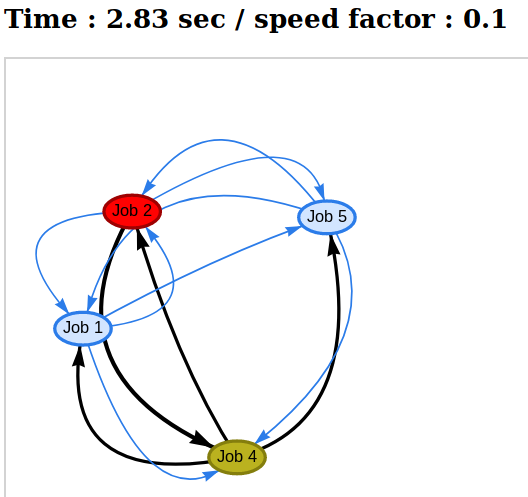
\includegraphics[width=0.4\linewidth]{figures/user_case/anim_pres.png}
        \caption{Timeline animation example}
        \label{fig:timeline}
      \end{figure}

      If we observe the leader election from the first result (without
      topology emulation and no crashes) with this tool, we will not see clearly
      the evolution of the nodes states, because the leader election finishes
      very quickly (< 8 ms) and it is hard to capture the visualisation of it
      (or with an very small speed factor).\\
      The main reason is the lack of latency between nodes. Indeed, without
      topology emulation, the RPC messages travel with the native latency
      (in case of the student installation, only docker network latency is
      expected), and then a candidate gets its vote granted really fast (and
      thus becomes the leader directly, with almost no chances of conflict
      with another node).

    \section{Robustness of solution}

      The student is not totally sure that his solution is correct, and he would
      like to try to break his Raft election by testing it with different
      network settings and by adding some fault injection in the critical
      parts of the process. Moreover, he wants to observe the difference of
      chances for a node to become leader depending on the network topology.

      \subsection{Network Topology Emulation}

        The student wants to test his implementation on different network
        topologies and see the difference of the chances for each node to
        become leader.

        \subsubsection{Topology settings}

          After testing the algorithm in a native network environment,
          the student tries it with three different network
          topology configurations, created with the network topology tool on
          the web application.\\
          Here are representations of the topologies~\ref{fig:topologies},
          with network specifications on the edges between nodes-routers and
          routers-routers.\\
          These specifications are focused on latency only,
          bandwidth constraints are not really influencing Raft election as
          it is using small and few packets.

          \begin{figure}[H]
            \centering
            \begin{subfigure}{0.6\textwidth}
              \centering
              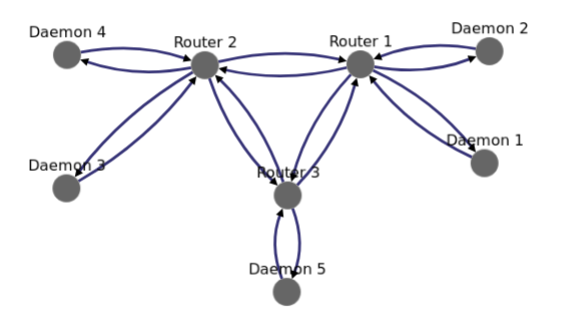
\includegraphics[width=1.0\linewidth]{figures/user_case/raft_topo_1.png}
              \caption{First topology - Normal: Router-Router -> 5 ms of delay and 10000kbps, Daemon-Router -> 15 ms od delay and 1500kbps}
              \label{fig:topo1}
            \end{subfigure}
            \centering
            \begin{subfigure}{0.6\textwidth}
              \centering
              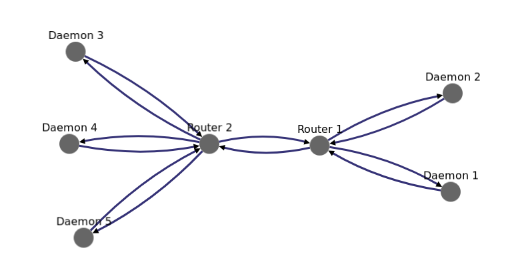
\includegraphics[width=1.0\linewidth]{figures/user_case/raft_topo_2.png}
              \caption{Second topology - Two sites: Router-Router -> 250 ms of delay and 15000kbps, Daemon-Router -> 10 ms od delay and 15000kbps}
              \label{fig:topo2}
            \end{subfigure}
            \centering
            \begin{subfigure}{0.6\textwidth}
              \centering
              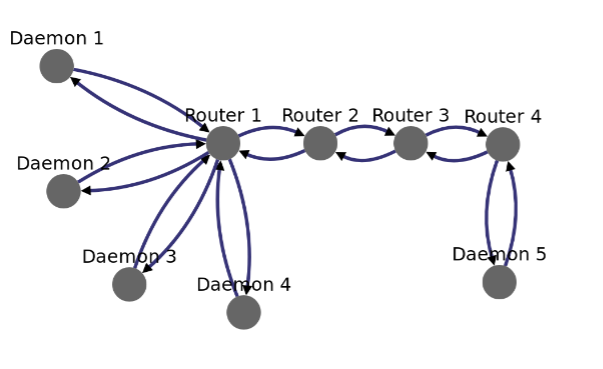
\includegraphics[width=1.0\linewidth]{figures/user_case/raft_topo_3.png}
              \caption{Third topology - Extreme: Router-Router -> 200 ms of delay and 15000kbps, Daemon-Router -> 15 ms od delay and 1000kbps}
              \label{fig:topo3}
            \end{subfigure}
            \caption{plots of three topologies}
            \label{fig:topologies}
          \end{figure}

        \subsubsection{Network Topology Impact}

          The student then tries his implementation with three network
          configurations~\ref{fig:topologies}.\\
          The log results shows that Daemons succeeded at achieving the leader
          election and quickly stabilize (one becomes the leader, the others
          are followers) in those different network configurations.\\
          But the network topology can affect the leader selection (some nodes
          have more chances than others of becoming the leader). He expects to
          obtain different results for each topology :

          \begin{itemize}
            \item First topology \ref{fig:topo1} : he expects that each node
            have almost the same chances to become the leader because the
            latencies between all endpoints is small compared to the timeout
            election range (1.5 seconds).
            \item Second topology \ref{fig:topo2} : he expects that daemons
            3-4-5 have slightly more chances to become the leader
            than daemons 1-2 because there is a kind of partition between the
            first two nodes and the rest with a big latency (250 ms).
            \item Thrid topology \ref{fig:topo3} : he expects that the daemon
            5 has very small chances to become the leader compared to the
            others (network packet take at minimun 0.63 second to travel between node 5 and other nodes).
            He expects also that the communication with daemon 5 always
            creates a RPC timeout (set to 0.5 second), and then other nodes will resend each
            time another packet to daemon 5.
          \end{itemize}

          To support these expectations and to test the fault tolerance of
          the algorithm, the student makes experiments with single fault
          injection. He adds a crash point in the heartbeat function to
          make the leader crash before the second heartbeat and
          thus trigger a new election :

          \begin{lstlisting}[style=MyLua]
...
function heartbeat()
  -- CRASH POINT 1 2 3 4 5: RECOVERY 0 : AFTER 1
  for i, n in pairs(job.nodes) do
...
          \end{lstlisting}

          The student launches the code turn during approximately 13 minutes,
          and parses the logs to get the number of times each node becomes the
          leader.\\
          First, he concludes that crashing the leader does not crashes the
          Raft election process but only restarts an election, as expected.
          He also obtains interesting result~\ref{tab:leader}, which at first glance,
          supports his expectations. \\
          Here, the purpose is \textbf{not} to make statistical evidence/model but
          only to show the importance of the topology emulation on a
          distributed algorithm and specifically of the chance of each node
          to become the leader during a Raft election process.\\
          But we can imagine scenarios of advanced studies to demonstrates
          the impact of certain network configurations on the leader election
          process thanks to \texttt{Splay}.\\

          \begin{table}[]
            \begin{tabular}{|c|c|c|c|c|c|c|}
            \hline
            Topologies             & \multicolumn{6}{c|}{\% Leader (number time become leader)}                                                                                                                                                                                                                                                                                                                         \\ \hline
            \multicolumn{1}{|l|}{} & Node 1                                                           & Node 2                                                          & Node 3                                                   & Node 4                                                  & Node 5                                                          & Total                                 \\ \hline
            Topology 1~\ref{fig:topo1}            & \begin{tabular}[c]{@{}c@{}}20.36 \%\\ (90)\end{tabular}          & \begin{tabular}[c]{@{}c@{}}21.27 \%\\ (94)\end{tabular}         & \begin{tabular}[c]{@{}c@{}}19.91 \%\\ (88)\end{tabular}  & \begin{tabular}[c]{@{}c@{}}18.78 \%\\ (83)\end{tabular} & \begin{tabular}[c]{@{}c@{}}19.68 \%\\ (87)\end{tabular}         & \begin{tabular}[c]{@{}c@{}}100 \%\\ (442)\end{tabular} \\ \hline
            Topology 2~\ref{fig:topo2}           & \textbf{\begin{tabular}[c]{@{}c@{}}10.50 \%\\ (38)\end{tabular}} & \textbf{\begin{tabular}[c]{@{}c@{}}9.67 \%\\ (35)\end{tabular}} & \begin{tabular}[c]{@{}c@{}}28.17\%\\ (102)\end{tabular}  & \begin{tabular}[c]{@{}c@{}}25.69 \%\\ (93)\end{tabular} & \begin{tabular}[c]{@{}c@{}}25.97 \%\\ (94)\end{tabular}         & \begin{tabular}[c]{@{}c@{}}100 \%\\ (362)\end{tabular} \\ \hline
            Topology 3~\ref{fig:topo3} & \begin{tabular}[c]{@{}c@{}}22.61 \%\\ (90)\end{tabular}          & \begin{tabular}[c]{@{}c@{}}25.63 \%\\ (102)\end{tabular}        & \begin{tabular}[c]{@{}c@{}}25.63 \%\\ (102)\end{tabular} & \begin{tabular}[c]{@{}c@{}}23.62 \%\\ (94)\end{tabular} & \textbf{\begin{tabular}[c]{@{}c@{}}2.51 \%\\ (10)\end{tabular}} & \begin{tabular}[c]{@{}c@{}}100 \%\\ (398)\end{tabular} \\ \hline
            \end{tabular}
            \caption{Result of Raft leader election after long run and by crashing the leader before the second heartbeart}
            \label{tab:leader}
          \end{table}

      \subsection{Advanced fault injection}

        The user already tested what happens in case of leader crashes, he now
        wants to increase his confidence in his implementation.\\
        Therefore, he injects other faults at different key points of the
        algorithm to see how his implementation will manage these faults.\\

        To achieve this, the student puts four crash points in his code.
        Ad before, he adds a crash point in the heartbeart function, but with
        other parameters (when the 6th heartbeart is called and recovers
        after 0.5 second) :

        \begin{lstlisting}[style=MyLua]
...
function heartbeat()
  -- CRASH POINT 1 2 3 4 5: RECOVERY 0.5: AFTER 5
  for i, n in pairs(job.nodes) do
...
        \end{lstlisting}

        Secondly, he adds acrash point not depending on the
        node state but triggering less often. It will be triggered by a node
        when it receives a vote request from a candidate with a probability
        of 0.05 :

        \begin{lstlisting}[style=MyLua]
...
function request_vote(term, candidate_id)
  -- CRASH POINT 1 2 3 4 5: RECOVERY 0.5: RANDOM 0.05
  print("RPC Request Vote FROM "..candidate_id.." Term: "..term)
...
        \end{lstlisting}

        As the third fault, he adds a crash point triggered when a vote is
        granted by a node :

        \begin{lstlisting}[style=MyLua]
...
if vote_granted == true then
  nb_vote = nb_vote + 1
  -- CRASH POINT 1 2 3 4 5 : RECOVERY 0.5 : RANDOM 0.06
...
        \end{lstlisting}

        And last, he places a crash point just \textbf{after} that a
        node replies to a vote request RPC.

        \begin{lstlisting}[style=MyLua]
...
        set_election_timeout() -- reset the election timeout
    end
    events.thread(function()
        -- CRASH POINT 1 2 3 4 5 : RECOVERY 0.5 : RANDOM 0.05
    end)
    return persistent_state.current_term, vote_granted
end
...
        \end{lstlisting}

        We create a new thread which will be executed after the RPC function
        returns, thus after the node sends it response (on network). Indeed this is
        working because of the non-preemptive nature of \texttt{Lua}, the thread
        will execute after the current one (RPC call), and the crash will happen (if happen)
        after the RCP response is sent back.\\

        After letting the code run on 5 daemons for 10 minutes, the student
        checks the logs for the different topology settings.\\
        He sees that everything went as expected. Indeed, the leader
        election process is performed without any problem and there is never
        more than on leader at the same time.\\
        Moreover, when there less than a majority of nodes is alive, the leader
        election process will not progress until there is a majority again.\\
        The student is now more confident about his implementation of Raft.

      \subsection{Animation results}

        Now the student has tried his Raft election implementation on
        different topologies and with some crash points, he can observe some
        interesting results thanks to the animation tool.\\
        A complete Raft election can be divided in multiple steps. The next
        figure shows a complete election process with a conflict between
        three candidates (candidates asking almost at the same time vote
        requests to the others).\\
        In this case, nobody gets the majority of votes, therefore another
        election will be triggered with a bigger term at some point.
        And with this new election, the candidate who received enough votes
        will become the leader (no conflict this time).\\
        Note that conflicts happen rarely with 3 candidates because the
        leader timeout is well-balanced thanks to randomization and the
        topology used is not an extreme case (topology 2 \ref{fig:topo2}).

        % Show four step of election: all followers -> two candidate -> one leader -> leader + heartbeat
        \begin{figure}[H]
          \begin{subfigure}{.45\textwidth}
            \centering
            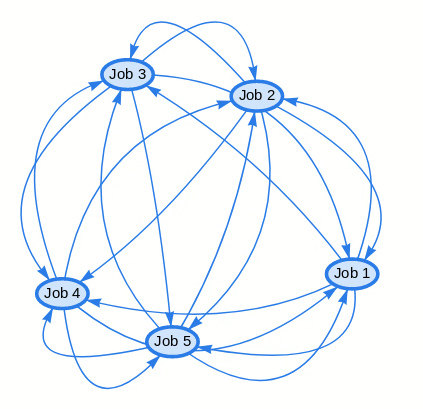
\includegraphics[width=1.0\linewidth]{figures/user_case/election_1.png}
            \caption{When all nodes are awaken and they are all followers (begin state)}
            \label{fig:ele1}
          \end{subfigure}\hspace{0.1\textwidth}
          \begin{subfigure}{.45\textwidth}
            \centering
            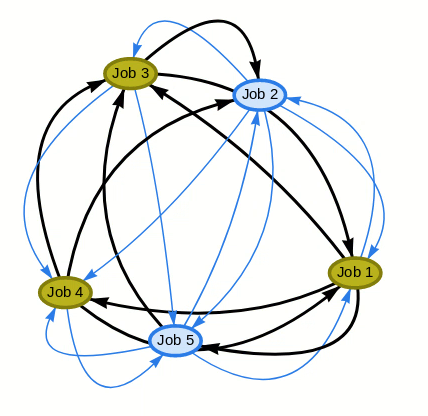
\includegraphics[width=1.0\linewidth]{figures/user_case/election_2.png}
            \caption{Three candidates for the leader job -> conflict, none become the leader, the majority is sliped}
            \label{fig:ele2}
          \end{subfigure}
          \begin{subfigure}{.45\textwidth}
            \centering
            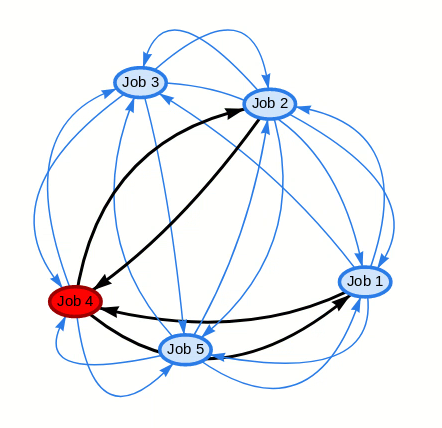
\includegraphics[width=1.0\linewidth]{figures/user_case/election_3.png}
            \caption{New leader election from job 4 with a bigger term -> becomes the leader when receives the majority}
            \label{fig:ele3}
          \end{subfigure}\hspace{0.1\textwidth}
          \begin{subfigure}{.45\textwidth}
            \centering
            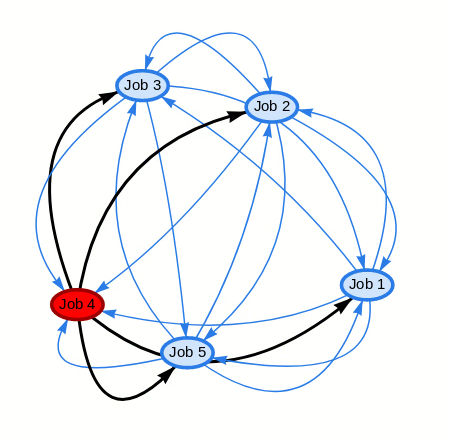
\includegraphics[width=1.0\linewidth]{figures/user_case/election_4.png}
            \caption{The leader (job 4) sending heartbeat to other nodes to avoid a new leader election}
            \label{fig:ele4}
          \end{subfigure}

          \caption{Raft election animation from the parsing of a job's log, with the topology in figure \ref{fig:topo2}
          and crash points for the leader when sending heartbeat}
          \label{fig:election}
        \end{figure}

        In case of figure~\ref{fig:election}, no node crashes but we can show
        that even when a crash happens, Raft is fault-tolerant as long as there
        is a majority of nodes alive (3 in this case). If there are only one or
        two nodes alive, the election can't be achieved until a third node
        wakes up.\\
        The animation shows that, when the leader crashed, one or multiple
        nodes triggered a new leader election process.\\
        Crashes can also happen on a follower or candidate node, which will not
        disturb the Raft process as long as there is a majority of nodes
        running.

  \chapter{Conclusion}

    We will first conclude this report by going through a list of improvements
    idea over the project, and then summarize our global achievements on the
    project compared to our initial objectives.

    \section{Improvements}

      This section will hold our thoughts about the further improvements
      that could be made on the project, these improvements are mainly about
      our new features, the improvements that could be made on the "legacy"
      services and also some improvements thoughts about the security.

      \subsection{New features improvements}

        Our new features on the \texttt{Splay} system may be improved over the future
        and we will expose our ideas and thoughts for each one of these
        features.

        \subsubsection{Lua editor}

        During the development of our features, we noticed that the Lua Editor
        is probably the less important one. The main reason making this feature
        the less important is that most of the time, users create their own Lua
        scripts on their favorite editor and then apply a copy-paste on the
        system.\\
        A fully integrated IDE with a Lua an installed Lua package offers more
        than our editor, but with little improvements, our editor could equal
        any other:

        \begin{itemize}
          \item \textbf{Basic Auto-Completion}: A basic auto-completion can be
          done for keywords (as any other IDE) and for named functions with
          the help of the Ace Editor package.
          \item \textbf{Specific Auto-Completion}: The integration of the \texttt{Splay
          Lua} library to the auto-completion feature with some hints would
          be a great achievement and make the Lua editor an even better
          option than an IDE.
          \item \textbf{Color Theme}: Ace allows to set a color scheme for
          the editor, an option for the user to change this color scheme
          might be a great option to make the development environment
          truly enjoyable.
        \end{itemize}

        As Ace can handle a lot of different languages, if in any further
        improvement a decision to switch the daemon technology was made (see
        next section about refactors), then it would be easy to change the
        targeted language.

        \subsubsection{Crash point}

          The crash point feature now handles two types of crashes and two
          behavior to adopt in case of a crash. This feature is very useful
          to simulate a hard stop of a machine (power loss, for example).\\

          However, we could improve this by adding new types of crashes like a
          network crash or network compartmentalization meaning that the
          nodes would still be running but could not communicate anymore
          with other nodes during the downtime.\\
          For this purpose, we could modify the socket wrapping done to achieve
          topology emulation (or creating a new one) where our crash library could ask
          for restrictions over the network simulation.\\
          Moreover, this idea can go futher, to be able to create network partition between
          several nodes, creating two or more splited network where nodes can
          only communicate with others located in the same partition.\\

          Moreover, we can imagine providing the user with more control options
          to configure more precisely what should happen in case of crash or
          when the crash should happen. For example, crashing when some
          precise conditions are met.

        \subsubsection{Topology Creation}

          The actual topology creation through the modern interface is very
          useful to build a precise topology in a quick way. However, we have
          a non-exhaustive list of ideas that could improve this feature, but
          wasn't achievable now because of time constraints:

          \begin{itemize}
            \item \textbf{Modifications of items on click}: For now, it is hard
            to modify existing edges, nodes or specs. The user needs to remove
            the specified item or modify it in the \texttt{XML} code, therefore
            an option to modify existing items through a form would be a good
            idea.
            \item \textbf{Edge in both directions}: Right now, the user can only
            add directed edges between nodes, adding an option to directly
            create edges in both directions would be a good idea and
            avoid double work with the directed edges through the form.
          \end{itemize}

      \subsection{Refactor of old services}

        We have rebuilt some parts of \texttt{Splay} using modern technologies as
        explained in the related section, but we have not made a complete
        refactor of the daemon and the controller. We think that those two
        services would need, in the future, a complete refactor or even be
        rewrote maybe using newer technologies. A database schema cleaning
        would also follow, as some fields of the various entities may not be
        useful anymore.

        \subsubsection{Daemon}

          The daemon is, with the controller, one of the most critical parts of
          the project and has been built using \texttt{Lua}~\cite{Lua}.\\
          During our work, after having stabilized the project, we encountered
          a lot of unused code lines, small bugs and code repetition in the
          Daemon codebase and we therefore carefully fixed those issues when
          encountered.\\
          Therefore, we reduced the usage of the \texttt{Splay} library by the Daemon
          and ended up with a lot of unused and undocumented code in this
          library. For these reasons, we think that a complete check of the
          \texttt{Splay Lua} library should be performed (with the help of a previous
          maintainer of the project) to provide it with helpful documentation
          that would ease its usage and would allow enhancing our busted test
          suite.\\

          Moreover, we saw by the end of the project that the socket
          topology restriction was not actually taking into account
          the packet loss rate and the queue length (maybe this feature was
          a work in progress in the latest version of the legacy codebase).\\
          Therefore, the topology settings that can be tweaked are limited to
          the bandwidth and latency.\\
          Furthermore, we saw that the topology restriction is based on the
          \textbf{IP} combined to a single port number, this causes unknown
          client sockets (because the port is different from the server port)
          and useless restrictions. For all these reasons, the socket topology
          (coming with the \texttt{SplayNet} module) needs to be improved.\\

          A radical solution to clean this service and offer a new alternative
          to users would be to completely rewrite the Daemon service using
          another technology.\\
          The best alternative for the language would be \texttt{Python}, \texttt{Python} is a
          very popular language with a supportive community and constantly
          updated, having rich libraries offering complete sets of tools.\\
          However, the main drawback of this solution would be the performance
          offered by vanilla \texttt{Python} compared to the very small core of Lua and
          its C integration. But the main drawback of Lua is evolution, Lua has
          not received major updates since 2014 and the libraries used in this
          project are not evolving too. Moreover, the tiny core of Lua forces
          the user to write its own basic functions that are built-in in many
          other languages and thus were placed in the \texttt{Splay} lib in our case.\\
          This results in a greater number of lines of codes for the \texttt{Splay} lib,
          which thus includes more chances of bugs.\\
          Going back to the performance question, using a just-in-time compiler
          such as \texttt{PyPy}~\cite{PyPy} to significantly boost the performance and
          using some distributed libraries to quickly create a new \texttt{Splay} library
          may be a solution.

        \subsubsection{Controller}

          The controller service is the brain of the project, it manages the
          different daemons, reads new data from the database and writes the
          results, dispatches the different jobs.\\
          Despite being such a central piece of the project, the code is still
          badly documented and still needs an advanced cleanup in its
          different parts, and it is also poorly tested even after we worked
          on it. We may, accordingly, propose two different ways to increase
          the quality and maintainability of the controller for future
          development phases:

          \begin{itemize}
            \item Using full object-oriented with sequel~\cite{Sequel} model
            object for each table of the database. The SQL queries are now
            raw ones which can be insecure (in case one forgets to manually
            check against injections) and which are hard to read.\\
            A sequel model object allows every operation on a SQL database
            through function calls in a nice a concise Ruby way, avoiding
            SQL error syntax and most importantly it is independent of the
            database management system.
            \item A meticulous refactor of some part of the controller may be
            a good idea, and more specifically the management of jobs sent to
            the daemons (a Ruby class named Jobd and its children classes), we
            indeed found most of the controller bugs in this part.
          \end{itemize}

      \subsection{Security Aspects}

        In the description of the legacy project, we saw that the user's job is
        supposed to be running in a restricted area and the project is secure in
        general.\\
        But with further analysis, we found out that the project was not secure
        in various ways:

        \begin{itemize}
          \item The restriction on the socket can actually be completely
          bypassed. Indeed, using Lua there is a way to unload a package
          dynamically (package.loaded["name\_package"] = nil). Using this
          technique, we can unload the socket package (that was loaded with a
          restriction) and reload it with the corresponding statements placed
          at the beginning of the job code and the restriction will not exist
          anymore.
          \item SQL calls in the controller are using string interpolation,
          in most of the cases, the call is secure manually adding escape
          characters in the string. Indeed, there is no security issue if
          each call is protected with escaping, but the fact that it is done
          manually is a bad practice and will create a security issue if
          any verification is mistakenly skipped by a developer.
        \end{itemize}

        We concluded that the installation of \texttt{Splay} needs to be only
        used by trusted people in a trusted environment. It is therefore
        extremely important for the project to have future work about the
        securitization of the platform so that it could be used everywhere.

    \section{Objectives Achievements}

      This project was a real challenge, we had to start working with an
      already existing project composed with multiple different services
      interacting in a complex way. We managed to understand the
      implementation details and habits of previous maintainers in order to
      achieve our goal of transforming \texttt{Splay} in an
      integrated platform for distributed systems training and learning.\\

      Our primary goal was to achieve a certain work of software engineering on
      the base project we started working with, which we accomplished with
      a solid test suite on the multiple services of the application.\\
      We wanted to improve the project structure and maintainability, which
      we did by reorganizing the code on different repositories, using
      the test suites with continuous integration to support further
      contributions. We revised the whole \texttt{Docker} management of
      the project, creating lightweight docker images with automatic
      builds on \texttt{DockerHub} and creating a \texttt{docker-compose} file
      for easy installation and set up of the project.\\

      Our main goal was to turn \texttt{Splay} in an integrated platform for
      distributed systems training and learning. We achieved this with a
      brand new web application using recent web technologies, and easy
      to use for students and professors. A complete Lua editor helps to
      write the distributed algorithm with syntax coloration and error
      parsing. A complete topology editor allows to draw complex network
      topologies on which running the distributed algorithms, and a fault
      injection system so that the user can trigger faults in specific
      parts of his implementation to test its robustness.\\

      Another idea for the project we had to put aside was to make the project
      run on a cluster of RaspberryPi. The cluster itself is a side-project
      and was not ready to receive a \texttt{Splay} installation at the
      time we finished this thesis.\\
      From our point of view, \texttt{Splay} still needs some refactoring
      of the oldest codebase so that it would completely support the
      implementations of new features and the improvements we listed before.\\

      We managed to show a real demonstration of a practical usage of
      \texttt{Splay} with the well-known Raft election algorithm, clearly
      presenting the importance, quality and usefulness of our contributions
      on the application. We are really satisfied about our result of our
      contributions on the application.

  \nocite{*}
  \bibliographystyle{plain}
  \bibliography{biblio.bib}

  % Back cover page
  \backcoverpage

\end{document}
